\documentclass[a4paper,10pt]{book}

\usepackage[utf8]{inputenc}
\usepackage[english]{babel}
\usepackage{euscript}
\usepackage{epigraph}

\usepackage{graphicx}
\usepackage{amsmath}
\usepackage{amssymb}
\usepackage{amsthm}
\usepackage{fancyhdr}



\usepackage{pictexwd,dcpic}

\usepackage{wrapfig}





%-------------- Margins
\setlength{\oddsidemargin}{20pt}
\setlength{\evensidemargin}{20pt}
\setlength{\marginparwidth}{-20pt}
\setlength{\textwidth}{400pt}
\setlength{\topmargin}{-10pt}
\setlength{\textheight}{600pt}

%--------------- Quotient
\def\quotient#1#2{%
	\raise1ex\hbox{$#1$}\Big/\lower1ex\hbox{$#2$}%
}

% ----------------- Argmin
\newcommand{\argmin}{\operatornamewithlimits{argmin}}

%------------ Theorems and maths --------
\theoremstyle{definition}
\newtheorem{definition}{Definition}[section]
%\theoremstyle{plain}
\newtheorem{example}{Example}[section]
\newtheorem{lemma}{Lemma}[section]
\newtheorem{observation}{Observation}[section]
\newtheorem{theorem}{Theorem}[section]
\newtheorem{prop}{Property}[section]
\newtheorem{corollary}[theorem]{Corollary}%[section]
\newtheorem{algorithm}{Algorithm}

%---------- Proof
%\newenvironment{proof}{\par\addvspace\topsep\noindent
%{\bf Proof:} \ignorespaces }{\qed}
%\newcommand{\qed}{\hspace*{\fill}$\Box$\ifmmode\else\par\addvspace\topsep\fi}


%------------ Norm
\newcommand{\euclideanMetric}[1]{\vert\lvert #1 \rvert\vert}
\newcommand{\supMetric}[1]{\vert\lvert #1 \rvert\vert_{sup} }

\newcommand{\quotes}[1]{\text{ \lq\lq  #1\rq\rq\phantom{z}}}


\RequirePackage{hyperref}
\hypersetup{ hidelinks=true}

\begin{document}


%%%%%%%%%%%%%%%%%%%%%%%%%%%%%%%%%%%%%%%%%%%%%%
%%%%%%%%%%%%%%%%INIZIO FRONTESPIZIO
\begin{titlepage}
%
\pagestyle{empty}
\begingroup
% INTESTAZIONE
\vspace*{-7\topskip}

\vspace{2 cm}

\begin{center}
        {\huge\bf \baselineskip=0.95em plus 1pt \expandafter{
        Toward a BCH-free Computation of the Composition of Stationary Velocity Fields
        \par}}
\end{center}

\vspace{0.5cm}
\begin{center}
	{\LARGE{Sebastiano Ferraris}\par}
\end{center}

%\vspace{2.5cm}

\vspace{2cm}
\begin{figure}[!h]
%centrare
\begin{center}
%resize in cm
\resizebox{4.0 cm}{4.0 cm}{
\includegraphics{figures/UCL_logo.jpg}} %1.5 2.5
\end{center}
\end{figure}
\vspace{1.3cm}

\begin{center}
	\LARGE{\rm\expandafter{Universtiy College London}}\par
	\expandafter{\Large{Medical Physiscs and Biomedical Engineering}\par}
\end{center}

\vspace{0.5cm}

\begin{center}
	A dissertation submitted in partial fulfillment 
	\\
	of the requirements for the degree of
	\\ 
	{\bf Master of Research}	
\end{center}

\vspace{0.2cm}
\begin{center}
	\today
\end{center}

\vspace{0.5cm}
%%\vspace{0.5cm}
%\begin{center}
%	{\LARGE{Tesi di Laurea Magistrale}\par}
%\end{center}

\begin{center}
\begin{tabular}{l p{3.3cm} l l}
	
	Supervisor& & Co-Supervisor \\
	\textbf{Tom Vercauteren} & & \textbf{Marc Modat}  \\
	
\end{tabular}
\end{center}


\vspace{1 cm}

%CHIUSURA

\par
\vfill\par 

\endgroup


\end{titlepage}

%%%%%%%%%%%%%%%%% PAGE JUMPERS:
%%%%%%%%%%%%%%%%%%%%%%%%%%%%%%%%%%%%%%%%%%%%

% \qquad
%  \thispagestyle{empty}
% \newpage
% \qquad
%  \thispagestyle{empty}
% \newpage

%\qquad
%  \pagestyle{empty}
% \newpage

 
%%%%%%%%%%%%  SOMMARIO


\qquad
\pagestyle{empty}
\newpage


% % % % % % % % % % % % % % % % % % % % % % % % % % % % % % % % % % % % % %
% % SUB SECTION
% % % % % % % % % % % % % % % % % % % % % % % % % % % % % % % % % % % % % %
\section*{Abstract}

Medical imaging employs techniques and tools belonging to several branches of mathematics and physics that, when applied to morphometric and statistical study of biological shape variability, are collected under the name of \emph{computational anatomy}. 
One of its critical tool, image registration, is widely used in both academical studies and applications, and continuously challenges researchers to enhance accuracy, improve reliability and reduce the time of the computations. The use of diffeomorphisms in image registration and the concomitant introduction of the log-euclidean framework to compute statistics, provide an interesting options to model the organs' deformations and to quantify the variations of anatomies.
One of the challenge of this setting are the numerical computation of the Lie exponential of stationary velocity fields (SVF), the Lie logarithm of the corresponding transformation and their combinations as they appear in the BCH formula: concept at the core of the underpinning theory of the \emph{log-demons} algorithm.\\
The necessity of finding fast numerical computation techniques of the BCH formula gave birth to the concept of log-composition presented in this thesis within some strategies for its computation.


% % % % % % % % % % % % % % % % % % % % % % % % % % % % % % % % % % % % % %
% % SUB SECTION
% % % % % % % % % % % % % % % % % % % % % % % % % % % % % % % % % % % % % %
\section*{Thesis' Organization}
%Four chapters, all alike in dignity are presented in this fair thesis: \\
\begin{enumerate}
	\item[{\bf Chapter \ref{ch:introduction}}] The first chapter is devoted to the introduction of diffeomorphic image registration and the main recent advancements. Here are introduced advantages and disadvantages of using diffeomorphisms as well as some of the milestone frameworks that led to, or are directly affected by the log-composition.
	
	\item[{\bf Chapter \ref{ch:tools}}] The second one is the chapter of mathematical elements and tools. We introduce main definitions and results from differential geometry directly involved in the proposed numerical methods, as Lie logarithm, Lie exponential, connections and parallel transport.
	The concept of log-composition, around which the research gravitates, is defined as consequence of the need of generalize the BCH formula, and we propose the first steps for its computation. 
	
	\item[{\bf Chapter \ref{ch:spatial_transformations}:}] In this section we introduce two sets of transformations on which the numerical methods will be tested and compared. The first set consists in the finite dimensional group of rigid body transformation of the plane: here logarithms and exponentials possess a closed form, therefore a ground truth to compare the methods is available.
	The second set of transformation on which numerical methods are applied are the set of diffeomorphisms corresponding to the infinite dimensional stationary velocity fields in the tangent space. For this second case no closed form are available, but comparing the exponential it is still possible to find a ground truth respect to which compare results.
	
	\item[{\bf Chapter \ref{ch:log_computations}:}] The algorithm to compute the logarithm (here called \emph{log-algorithm}) presented in \cite{Bossa2007} is grounded on the BCH formula and can be cleanly reformulated using the log-composition. Each numerical method to compute the log-composition become naturally available to challenge its performance.
  
	\item[{\bf Chapter \ref{ch:results}:}] Here we are at the experimental results. The log-composition applied to rigid and diffeomorphic registration is applied to synthetic data and clinical images. \\
	
	
\end{enumerate}











%%%%%%%%%%%%  INDICE

\pagestyle{plain}  \pagenumbering{Roman}
\tableofcontents



%%%%%%%%%%%%%%%%%%%%%%%%%%%%%%%%%%%%%%%%%%%%%%%%
%%%%%%%%%%%%%%%%%%%%%% CAPITOLI     %%%%%%%%%%%%%%%%%%%%
%%%%%%%%%%%%%%%%%%%%%%%%%%%%%%%%%%%%%%%%%%%%%%%%

\newpage
\pagestyle{fancy} \pagenumbering{arabic}


\fancyhead{} % clear all header fields

\fancyhead[LE]{\slshape \rightmark}

\fancyhead[RO]{\slshape \leftmark}
\fancyfoot[C]{\thepage}
\renewcommand{\headrulewidth}{0.4pt}
%\renewcommand{\footrulewidth}{0.4pt}


%\fancyhead[RO,LE]{\bfseries The performance of new graduates}
%\fancyfoot{} % clear all footer fields
%\fancyhead[LE,RO]{\thepage}
%\fancyhead[LO]{\thesection}
%\fancyhead[RE]{\thechapter}
%%\fancyfoot[CO,RE]{To: Dean A. Smith}
%\renewcommand{\headrulewidth}{0.4pt}
%%\renewcommand{\footrulewidth}{0.4pt}



\chapter{Image Registration Framework}\label{se:registration_framework}

\begin{flushright}
	\emph{Play only the neccessary notes. The other, try not to play them. \\ -João Gilberto}
\end{flushright}


% % % % % % % % % % % % % % % % % % % % % % % % % % % % % % % % % % % % % %
% % SUB SECTION
% % % % % % % % % % % % % % % % % % % % % % % % % % % % % % % % % % % % % %
\section{Introductory Definitions}
A \emph{$d$-dimensional image} is a continuous function from a subset $\Omega$ of the coordinate space $\mathbb{R}^{d}$ (having in mind particular cases $d=2,3$) to the set of real numbers $\mathbb{R}$. Given two of them, $F : \Omega_{F}  \rightarrow\mathbb{R} $ and $M : \Omega_{M}  \rightarrow\mathbb{R} $, called respectively \emph{fixed image} and \emph{moving image}, the \emph{image registration problem} consists in the investigation of features and parameters of the transformation function
\begin{align*}
\varphi :\mathbb{R}^{d} \supseteq \Omega_{F} & \longrightarrow \Omega_{M}\subseteq \mathbb{R}^{d}   \\
\mathbf{x} &\longmapsto \varphi (\mathbf{x}) 
\end{align*}
such that for each point $\mathbf{x}\in \Omega_{R} $ the element $M(\varphi (\mathbf{x}))$ and $F(\mathbf{x})$ are closed as possible according to a chosen metric. The function $M\circ\varphi $ is called \emph{warped image}.\\
The underpinning idea can be represented by the following diagram, where $\varphi$ is the solution that makes $f$ the identity function.

\[
\begindc{\commdiag}[40]
\obj(-30,30)[Or]{$\Omega_{F}$}
\obj(0,30)[Ot]{$\Omega_{M}$}
\obj(-30,10)[Rref]{$\mathbb{R}$}
\obj(0,10)[Rtarg]{$\mathbb{R}$}

\mor{Or}{Ot}{$\varphi$}
\mor{Or}{Rref}{$F$}
\mor{Ot}{Rtarg}{$M$}
\mor{Rref}{Rtarg}{f}[1,1]

\enddc
\]
% fine diagramma

\noindent
This definition leave two degrees of freedom in searching for a solution: the domain of the transformation (also called deformation model), and the metric to measure the similarity between images. \\
Once these are chosen, they can be used as constituent of an \emph{image registration framework}: an iterative process that at each step provides a new function $\varphi$ that approaches $f$ to the identity.
Additional degrees of freedom can be defined in a refined framework: the metric can be considered with an additive regularization term, that introduces a constraint based on prior knowledge about the searched solution:
\begin{align}\label{eq:general_cost_function}
\mathcal{O}(F, M, \varphi) = \text{Sim}(F,M,\varphi) + \text{Reg}(\varphi) 
\end{align}
where $\text{Sim}$ is a function that measure the similarity, while $\text{Reg}$ is the regularization term.
Other two degrees of freedom are optimization algorithm on which the optimizer is based and the resampling - process of resize the image from one dimension to another - strategy. It can be chosen over several possibilities (nearest neighborhood, linear, cubic, ...).

% % % % % % % % % % % % % % % % % % % % % % % % % % % % % % % % % % % % % %
% % SUB SECTION
% % % % % % % % % % % % % % % % % % % % % % % % % % % % % % % % % % % % % %
\section{Iterative Registration Algorithm}

The definition of registration problem and the iterative algorithm described raise several issues. For example there are no reasons to believe that such a correspondence is unique and that there is at least one of them whose behaviour corresponds to a reasonable biological transformation between anatomies. One way to deal with this problem is tp add some constraints on the transformation $\varphi$, such that it models realistic changes that can occur in biological tissues. The kind and quality of the constraints are one of the feature that distinguish registration algorithms one from the other. \\
Conscious of the risk involved in any rigid classification, in particular when about rapidly evolving fields, we can see the image registration framework as a device with some knobs, each with its range:
\begin{align*}
\varphi &\in \{ \text{Transformations }\}\\
\text{Sim} &\in \{ \text{Similarity measures }\}\\
\text{Reg} &\in \{ \text{Regularization Terms }\}\\
\text{Res} &\in \{ \text{Resampling techniques }\}\\
\end{align*}
and with an optimization technique, borrowed from the various from literature, as gradient descent, aimed to optimize the sum of the similarity and the regularization.
Under the hood of this ideal device we may see something that can be schematically represented as in figure \ref{fig:iterative_algorithm_scheme}.

\begin{figure}[!ht]
	\centering
	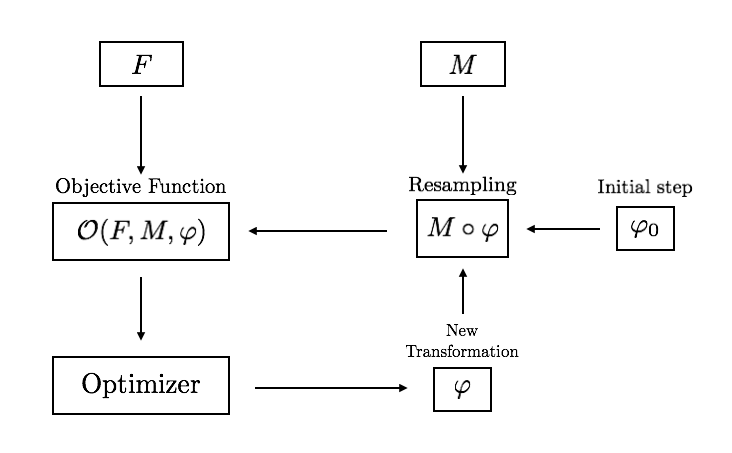
\includegraphics[scale=0.35]{figures/iterative_algorithm.png}
	\caption{Image registration framework scheme.}
	\label{fig:iterative_algorithm_scheme}
\end{figure}

\noindent
Just from this simplified scheme we can see that at each step moving and fixed images are defined within their domain, not necessarily coincident. 
It is always possible to define a common domain $\Omega = \Omega_{R}$, called  \emph{background space}, on which both of the images are defined.
%Avoid the resampling at each iteration decreases computational time, reduces artifacts and enable to have more control on the consequence of the chosen resampling technique.
%
%\begin{figure}[!ht]
%	\centering
%	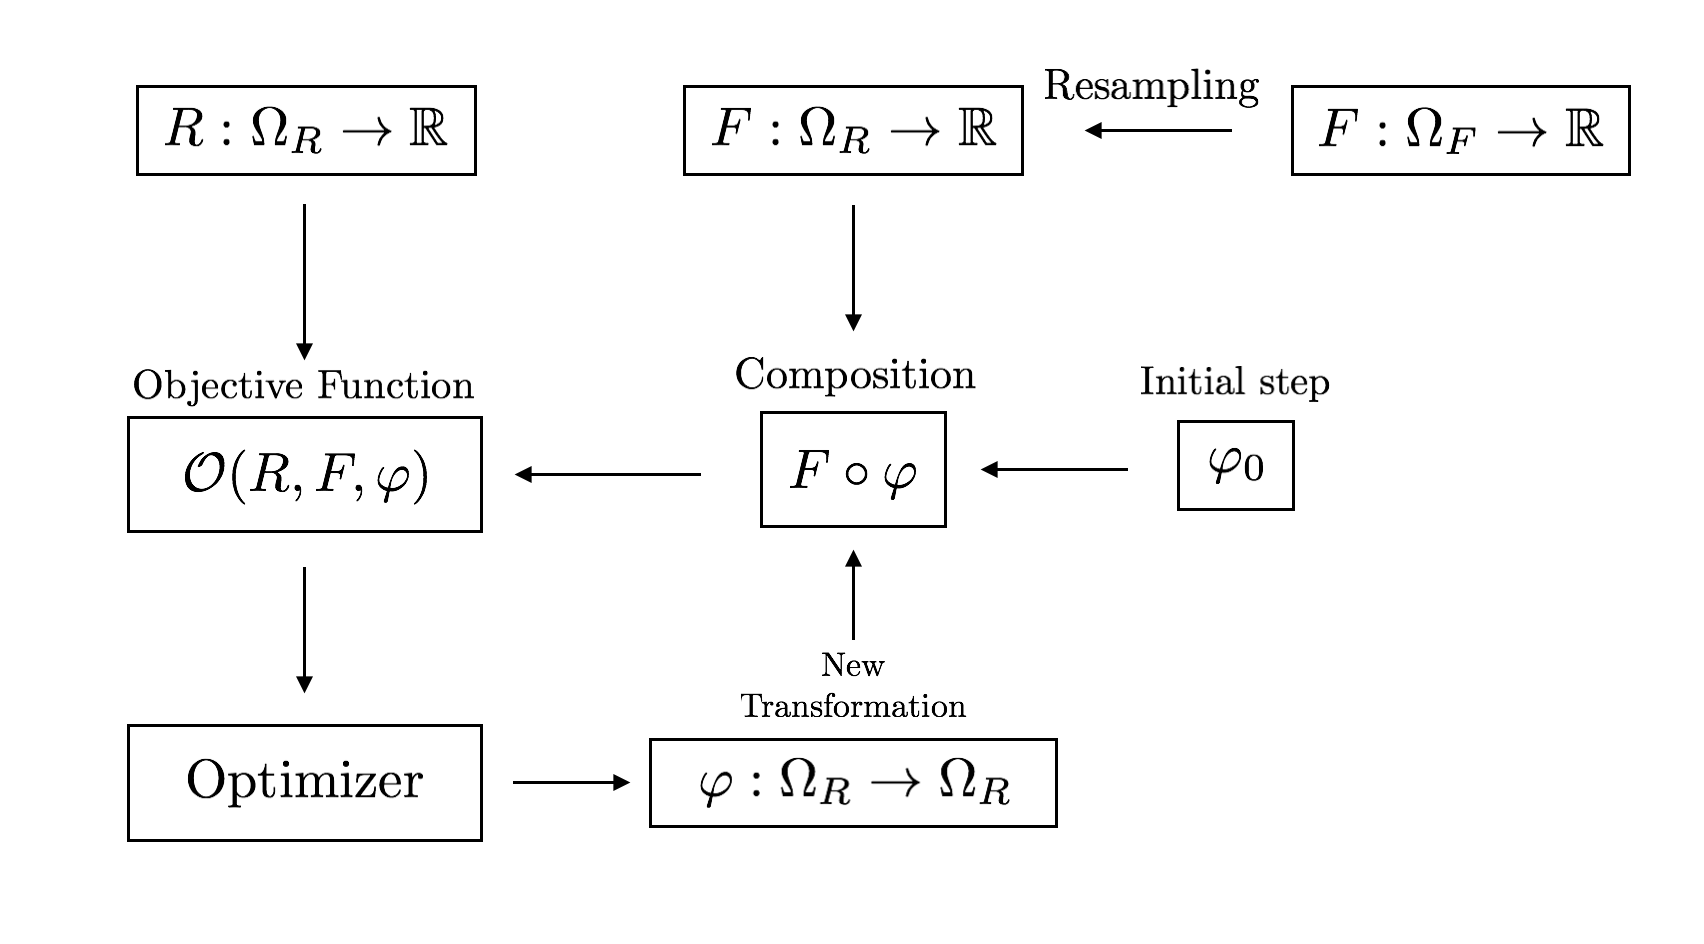
\includegraphics[scale=0.35]{figures/iterative_algorithm_res.png}
%	\caption{Image registration framework scheme.}
%	\label{fig:iterative_algorithm_scheme_modified}
%\end{figure}
\noindent
Far from being a complete overview of all of the possible framework does not take into account the fact that each version or implementation inevitably involves different needs and consequent challenges. Solutions found for each case may fall outside this simplification scheme: for example the parametrization of the transformations (or the deformation field's update) at each iterative step do not appear in this picture, even though is a fundamental feature. \\
In the following section we will going from the generalized framework to some specific aspects: we are interested in performing numerical computation to compute diffeomorphisms (bijective differentiable maps with differentiable inverse\footnote{Take the real valued $f(x)=x^3$: is bijective differentiable but the inverse is not everywhere differentiable.}). They are particularly appealing in medical imaging since in many situation biological modification do not involve any change in tissues' topology. We will see some details of parametrization of diffeomorphisms in five different frameworks: the LDDMM, the Shooting LDDMM, the Stationary LDDMM (or SVF), the DARTEL and the Demon.  In addition some details about the implementation of the image registration toolbox NiftyReg, used for some experiments in this research, can be found in the appendix.\\
Recent surveys in image registration can be found in \cite{Sotiras:survey:13} and \cite{Hill:survey:01}.

% % % % % % % % % % % % % % % % % % % % % % % % % % % % % % % % % % % % % %
% %  SECTION
% % % % % % % % % % % % % % % % % % % % % % % % % % % % % % % % % % % % % %
\section{Using Diffeomorphisms: Utility and Liability}

Idea of using diffeomorphisms can originate from two different perspective: if we imagine motion of captured images as motion of a fluid, we will start to approach the model using fluid dynamics; if we image motion as optical flow we will rely on differential geometry. Remarkably medical imaging application reveals common aspects of both underpinning theories, and requires some more since the discrete nature of actual input and output.\\
If we consider the rigid body transformation from classical mechanics, our transformations will be elements in $SE(3)$, the Lie group defined by combination of spatial rotations and translations. Five degrees of freedom, he possesses are enough to align 3d images; for continuous motions that maintains anatomical features between images they are not. We consider the Lie group of diffeomorphism $\text{Diff}(\Omega)$.
As already said, these functions are particularly appealing in computational anatomy since their topology-preserving nature, but their mathematical formalization has encountered many issues.\\ 
Attempt to provide this object some handle to manipulate it easily was done for the first time in 1966 in \cite{arnold1966geometrie}: to solve differential equation in hydrodynamic  $\text{Diff}(M)$ is considered as a Lie group with its Lie algebra. This assumption is not formally prosecuted in accordance to the problem-oriented nature of this paper\footnote{Subsequent steps in the exploration of the set of diffeomorphisms as a Lie group are \cite{marsden1970hamiltonian} and \cite{leslie1983lie}, \cite{omori1970group}. A survey on early development of infinite dimensional Lie group can be found in \cite{milnor1984remarks}.}.
The initial idea to consider $\text{Diff}(M)$ as a differentiable manifold involves to have it locally in correspondence with some generalized \lq\lq infinite-dimensional euclidean \rq\rq space. Attempt to set this correspondence showed that for some infinite-dimensional group the transition functions are smooth over Banach spaces. This led to the idea of Banach Manifolds. Unfortunately the group of diffeomorphisms do not belongs to the category of Banach manifold but requires a more generals space on which the transition map are smooth: the Frechet spaces. 
Thus the approach to the mathematical formalization of the general infinite dimensional Lie group involves Frechet differentiable manifolds. In this space we do not have anymore important theorems from analysis, as the inverse function theorem, or the main results from the Lie group theory in a finite dimensional settings, as Lie correspondence theorems.\\
These difficulties led some researcher in approaching the set of diffeomorphisms from other perspectives: for example, instead of treating $\text{Diff}(M)$ as group equipped with differential structures it is seen as a quotient of other well behaved group \cite{wojtynski1994one}.\\
Without denying the importance of fundamentals and underestimating the doors research in this domain may open, we will approach the matter in as similar way of what has been done in set theory: we will use a naive approach to infinite dimensional lie group, where the fundamental definition of infinite dimensional Lie group is a generalization of the finite dimensional case left to the intuition. 
We work then mostly on finite dimensional settings, relying on important theorems and easy close formulas, and we will extend methods and results developed here in the infinite case -clearly - with proper precautions.

%Besides, our purpose is not 'generalize definitions and theorems, while dodging counterexamples, but rather use the transformation groups for practical applications.


% % % % % % % % % % % % % % % % % % % % % % % % % % % % % % % % % % % % % %
% % SUB SECTION
% % % % % % % % % % % % % % % % % % % % % % % % % % % % % % % % % % % % % %
\subsection{LDDMM}

LDDMM \cite{beg2005computing} framework originates by considering motion between images as the motion of a fluid, and borrows its analytic tools from fluid dynamics. In this context the full set of homeomorphisms $\text{Hom}(\Omega)$ (continuous function from the background space $\Omega$ to itself with continuous inverse) is considered as a group with the composition. This group act\footnote{In this action it is preferable to consider the composition with the inverse, because this same action in differential geometry, called pull-back play the role of the contravariant operator of the push-forward, widely used to make a vector field act on a domain different from the one has been originally defined.} on the set of images defined on the background space $\mathcal{I}_{\Omega}$ as
\begin{align*}
\text{Hom}(\Omega) \times \mathcal{I}_{\Omega} & \longrightarrow  \mathcal{I}_{\Omega}   \\
(\varphi,F) &\longmapsto F\circ \varphi^{-1}
\end{align*}
The orbits of the subgroup of diffeomorphisms $\mathbb{G}$ on the image $F$, defined as
\begin{align*}
\mathcal{O}_{\mathbb{G}}(F) = \{ F\circ \varphi^{-1} \mid \varphi \in \mathbb{G} \}
\end{align*}
consists on all the images having the same topology\footnote{The idea of having the same topology is an analytical consequence of the definition of diffeomoprhism. Separated domains remains separated, although if they gets close enough, let say that their distance is less than the size of a voxel for a significant region, then the discretization will not maintain analytical topology and could broke it anyway.} of $F$.\\
In consequence of this, the Similarity term will be the distance between the moving image and the fixed image in the same orbit:
 \begin{align*}
 \text{Sim}(F,M,\varphi) = \frac{1}{\sigma^2}\euclideanMetric{F(\varphi^{-1})  - M  }_{L^{2}}^{2}
 \end{align*}
To define the regularization term that provides the optimal $\varphi$ at each step, in LDDMM (and subsequent frameworks) is considered the norm of the velocity vector field tangent to the transformation. Limiting is length means limiting the speed of the transformation at each step.
We consider a generic time varying vector field (TVVF) as the continuously differentiable map 
\begin{align*}
v:[0,1] & \longrightarrow  \text{Vect}(\Omega)\\
t  &\longmapsto  v_{t}  : \Omega \longrightarrow   \mathbb{R}^{d} \\
& \qquad \quad \quad \mathbf{x} \longmapsto v_{t}(\mathbf{x} )
\end{align*}
where $\text{Vect}(\Omega)$ is the set of all of the vector field over $\Omega$. With this notation $v$ is a vector field that changes continuously over a time parameter defined between $0$  and $1$. Once initial conditions are given, at each TVVF, corresponds a time varying homomorphisms defined  by the following ODE 
\begin{align}\label{eq:ode_phi_v}
\frac{d\phi_{t} (\mathbf{x})}{dt} = v_{t}(\phi_{t}(\mathbf{x} ))
\end{align}
where 
\begin{align*}
\phi : [0,1] & \longrightarrow  \text{Hom}(\Omega)\\
t  &\longmapsto \phi_{t}  : \Omega \longrightarrow    \Omega \\
& \qquad \quad \quad  \mathbf{x} \longmapsto \phi_{t}  (\mathbf{x} )
\end{align*}
Now the transformation $\varphi$ between fixed and moving images ($ R\circ \varphi^{-1} = T $) in which we where originally interested, can be defined within the couple $(v_{t},\phi_{t})$.  For $t = 0$, $\phi_{t} = Id$, identity of the group of homeomorphisms, and for $t = 1$, $\phi_{t} = \varphi$:
\begin{align*}
\varphi = \phi_{1} = \phi_{0} + \int_0^1 v_{t} (\phi) dt
\end{align*}
The set $\{ v_{t} (\phi) \mid t \in \lbrack 0,1 \rbrack \}$ is a path of transformations that varies continuously over the parameter $t$, starting at the identity and ending in the one the registration framework is looking for.\\
To have an efficient algorithm and a meaningful constraint on the resulting transformation, it is reasonable to consider $\phi_{t}$ as the shortest path between the identity and $\varphi$, so to have $v_{t} $ as the one that makes minimal the distance between transformations\footnote{This next equation can provide a metric on the manifold of the transformations, making it a Riemannian manifold. On the other side starting with a metric previously defined on the manifold, the consequence existence of geodesics may avoid the computation of the inf. In both cases this \lq\lq Riemannian approach\rq\rq  makes unavoidable the passage toward a metric, and makes the LDDMM a metric based algorithm.}:
\begin{align*}
l = \inf_{v_{t} ~ : ~ \dot{\phi_{t}} (\mathbf{x}) = v_{t}(\mathbf{x} )}  \int_{0}^{1} \euclideanMetric{v_{t}}_{L^2}^{2}dt
\end{align*}
In the LDDMM, ending points of path on the set of diffeomorphisms, whose tangent vector field (that varies over time) and can be used as regularization term:
\begin{align*}
\text{Reg}(F,M,\varphi) =  \int_0^1  \euclideanMetric{L v_{t} }_{L^{2}}^{2}  dt
\qquad 
\dot{\phi_{t}} (\mathbf{x}) = v_{t}(\mathbf{x} ) 
\quad 
\phi_{0} = Id
\quad 
\phi_{1} = \varphi
\end{align*}
Were $\varphi$ in the registration framework is the one provided by the optimization algorithm at the previous step, and $L$ is a linear operator that can be dependent on some parameters that makes the approach even more general\footnote{Recent approaches more image-oriented, proposed to use a kernel instead of an Operator.}. The operator $L$ is defined as $L = (\alpha\nabla + \gamma)$ for $\alpha$ and $\gamma$ real parameters and $\nabla$ the Laplace operator.\\
From the differential equation \ref{eq:ode_phi_v}, and in consequence of the definition of $\varphi$ the optimization function \ref{eq:general_cost_function} is defined as:
\begin{align*}
 \argmin_{v_{t} ~ : ~ \dot{\phi_{t}} (\mathbf{x}) = v_{t}(\mathbf{x} ) } 
\mathcal{O}(F, M, \varphi) 
= 
\argmin_{v_{t} ~ : ~ \dot{\phi_{t}} (\mathbf{x}) = v_{t}(\mathbf{x} ) } 
\int_0^1 \euclideanMetric{L v_{t} }_{L^{2}}^{2} dt + \frac{1}{\sigma^2}\euclideanMetric{F(\varphi^{-1})  - M  }_{L^{2}}^{2}
\end{align*}
And so the optimizer, at each step of the registration will look for
\begin{align*}
\hat{v} 
= 
\argmin_{v_{t} ~ : ~ \dot{\phi_{t}} (\mathbf{x}) = v_{t}(\mathbf{x} ) } 
\int_0^1 \euclideanMetric{L v_{t} }_{L^{2}}^{2} dt + \frac{1}{\sigma^2}\euclideanMetric{F(\varphi^{-1})  - M  }_{L^{2}}^{2}
\end{align*}
With this definition we see that is the $TVVF$, instead of the transformation $\varphi$, to be the output of the registration algorithm. On the computational side this appears even more natural in software implementation, the action of a diffeomorphisms $\varphi$ on an image is easily computed if the transformation is provided in term of discretized vector field $v_{t}$. \\
If $G$ is a cubic grid defined as the discretization of the background space $\Omega$, then a vector field dependent on time is parametrized as a 5-dimensional matrix
\begin{align*}
A = A(x,y,z,t,d) \qquad (x,y,z)\in G , ~~ t \in \lbrack 0,1\rbrack  ~~ d = 1,2,3
\end{align*}
where $(x,y,z)$ are discrete position of the grid, $t$ is the time parameter and $d$ is index of the coordinate axis. So the tangent vector $\mathbf{v}_{\tau}(x_0,y_0,z_0)$ at the point of the grid $(x_0,y_0,z_0)$, at time $\tau$, has Cartesian coordinate
\begin{align*}
\mathbf{v}_{\tau}(x_0,y_0,z_0) = (A(x_0,y_0,z_0,\tau,1), A(x_0,y_0,z_0,t,2), A(x_0,y_0,z_0,\tau,3))
\end{align*}
In the LDDMM approach, each transformation, in particular input and output of the optimization algorithm are discretized time varying velocity fields; the update at each step is given by
\begin{align*}
\mathbf{v}^{k+1} = \mathbf{v}^{k} - \epsilon \nabla d\mathcal{O}
\end{align*}
where $\mathbf{v}^{k}$ is the $k$-th step of the approximation, $d\mathcal{O}$ is the discretized version of the optimization function and $\epsilon$ is the gradient descent step size.
Details of the algorithms are provided in \cite{beg2005computing}; for purpose of this thesis it is important to notice that diffeomorphisms are used for the underpinning theory, as the solution of the differential equation \ref{eq:ode_phi_v}, and they are considered in the implementation while computing the similarity function; they are not used to compute the update at each step.

% % % % % % % % % % % % % % % % % % % % % % % % % % % % % % % % % % % % % %
% % SUB SECTION
% % % % % % % % % % % % % % % % % % % % % % % % % % % % % % % % % % % % % %
\subsection{Shooting LDDMM}

A direct upgrade of the 

Euler poincare equation to compute the momentum equation.


Only geodesics with initial condition.


\cite{vialard2012diffeomorphic}




% % % % % % % % % % % % % % % % % % % % % % % % % % % % % % % % % % % % % %
% % SUB SECTION
% % % % % % % % % % % % % % % % % % % % % % % % % % % % % % % % % % % % % %
\subsection{Stationary Velocity Fields LDDMM}



The approach of using time varying velocity field (TVVF) is a consequence of the differential equation involved in the registration problem. Solutions to differential equation depends on time. Another approach, is to start from the manifold structure on which the solution lives, the integral domain. In this context higher terms of differential equations are element of the tangent bundle. These objects do not originates from any differential equation, and retain their dignity of vector field even if independent form time parameters. The first time the passage form TVVF as solution to differential equation, to SVF as elements living in the tangent bundle of the integral domain of differential equation was done in \cite{arsigny2006log}. Using SVF in image registration algorithms have many advantages: a greedy strategy is adopted, so that at each iteration an update only of the stationary velocity field is computed and added to the one of the previous step. This makes the algorithm faster and less memory consuming. On the other side we have two main drawback: the possibility to perform statistics on SVF become less straightforward and the set of SFV is a subset of the diffeomorphisms with no group structure. More details on this will be seen in section \ref{se:svf_set}.

xxx parametrization of SVF

xxx the discretization

xxx the composition of SVF 

xxx how statistics can be performed relying on the tangent spaces


% % % % % % % % % % % % % % % % % % % % % % % % % % % % % % % % % % % % % %
% % SUB SECTION
% % % % % % % % % % % % % % % % % % % % % % % % % % % % % % % % % % % % % %
\subsection{DARTEL}


% % % % % % % % % % % % % % % % % % % % % % % % % % % % % % % % % % % % % %
% % SUB SECTION
% % % % % % % % % % % % % % % % % % % % % % % % % % % % % % % % % % % % % %
\subsection{Log-Demon}

In daemonology 

Dartel, LDDMM shooting, do not requires any log composition.
Log-composition is used in the 
1) Log-demon  - Tom
2) Bossa algorithm
3) Log euclidean by arsigny
4) Schild's Ladder - marco



In fact, given two TVVF $u_t$ and $v_t$ there is no straightforward operation that provides the TVVF that corresponds to the composition of the diffeomorphisms that generates these TVVF. To compute this, the vector field must be integrated to obtain the corresponding transformation $\psi$ and $\phi$. Corresponding transformation must be then composed and derived, to obtain again a TVVF that corresponds to the tangent vector field of the composition of $u_t$ and $v_t$.



% % % % % % % % % % % % % % % % % % % % % % % % % % % % % % % % % % % % % %
% % SECTION
% % % % % % % % % % % % % % % % % % % % % % % % % % % % % % % % % % % % % %
\section{Stationary Velocity Fields and the Composition of Diffeomorphisms in the Tangent Space}

% why do we need compositon of diffeomorphisms in diffeomorphic image registration. Why it is such a crucial thing and why it is difficult.
% Heay computations involved, lack of a close formula, and so on... The task is hard but we are brave enough to try!!

\noindent
xxx computational anatomy and the need for statistics.

\noindent
xxx introduction of log and exp concepts (formally later, in section \ref{se:lie_exp_log_comp} ).

\noindent
xxx starting from vectors, ending with one vector: the log composition, idea, not formally defined.

\noindent
defined as the vector $\mathbf{w}$ in the Lie algebra $\mathfrak{g}$ that reflects the composition in the Lie group of two vectors $\mathbf{u}, \mathbf{v}$ in the same tangent space:
\begin{align*}
\mathbf{w} = \log(\exp(\mathbf{u})\circ\exp( \mathbf{v}))
\qquad
\forall \mathbf{u}, \mathbf{v} \in \mathfrak{g}
\end{align*}


\noindent
xxx the BCH formula, as the first method to compute the log-composition.











%Under this light, the transitions from the Lie group to Lie algebra (the Lie logarithm) and its return (the Lie exponential) become fundamental tools.
%The main topic of this research is the evaluation of the operation that we define here as \emph{Lie algebra Group Composition}, or simply \emph{Group Composition}, 
%
%
%
%
%One of the Matrix Lie group explored in this research is the special euclidean group $\text{SE}(d)$, or group of rigid transformations.
%A little increase in the number of degrees of freedom leads to the group of the affine transformations, where scaling and shearing have been added to the possible transformations. \\
%The idea of maximize the number of degrees of freedom in a transformation that maintains anatomical features between images, led to consider the Lie group of diffeomorphism $\text{Diff}$.
%A diffeomorphism $p$ can be expressed as the sum of the identity function with a differentiable transformation depending on $\mathbf{x}$. It is possible to write:
%\begin{align*}
%p(\mathbf{x})  = \mathbf{x} + \gamma(\mathbf{x})
%\end{align*}
%With this notation the vector $\dot{\gamma}(\mathbf{x})$ is the speed\footnote{as we will see, a feasible way to express a set of diffeomorphisms is as the solution of the differential equation defined by the velocities of the transformation.} of each point from its original to a new position due to the application of $p$.\\
%In the iterative diffeomorphic registration algorithm (in which the structure is defined by regularization and similarity), to obtain the update at each step, it is required to apply consecutively two diffeomorphisms $p_{i}$ and  $\hat{p}_{i+1}$ and consider the resulting composition as the required update.
%%\begin{figure}[!ht]
%%	\centering
%%	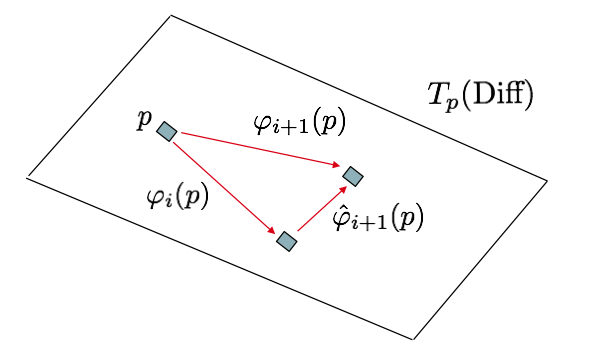
\includegraphics[scale=0.35]{figures/diff_update.png}
%%	\caption{Composition of tangent vectors of diffeomorphism (provisional).}
%%	\label{fig:composition1}
%%\end{figure}
%As a consequence, the corresponding vector of the transformation $p_{i+1}$ in the tangent space of the Lie group can be computed, given two vectors in the tangent bundle, with an operation called here \emph{the group composition in the Lie algebra}.\\
%In \cite{Bossa2007} the BCH formula appears as an improvement of the scaling and squaring algorithm to compute the logarithm of a matrix. As noticed in the same paper, the BCH formula is used in a infinite dimensional settings, while its validity has been proven only for finite dimensional Lie group. In addition while composing the logarithm of a composition of two exponentials, the initial tangent vectors belongs to the same tangent space. This is not the case while composing $p_{i}$ with $\hat{p}_{i+1}$ the tangent vector that defines $\hat{p}_{i+1}$ is an element of the tangent plane to $p_{i}$. \\
%Is it possible to reach a proper computation thanks to the definition of Affine exponential, that differs from the Lie exponential used in \cite{Bossa2007} .
%
%
%
%
%
%
%The BCH formula provides an expression of the Group Composition in the finite dimensional case expressed as an infinite series of nesting commutators. The difficulties involved in dealing with this formula, as well as its non completely proper use in the infinite dimensional setting, gave birth to some methodologies and approaches, whose investigation is the main goal of this research. One of these approaches, involves the Taylor expansion and has a computable form in the finite dimensional. A geometrical approach that holds also in the infinite dimensional case is the parallel transport.
%It can be considered as a natural approach to evaluate the group composition with offset. It consists in the transport of the vector $\mathbf{v}$ along the geodesic having $\mathbf{u}$ as tangent vector such that during the transport it maintains the condition of parallelism. The resulting vector $\mathbf{v}^{\parallel}$ in the tangent plane of $\mathbf{u}$ can be then summed with $\mathbf{v}$ with similar results to the direct application of the BCH. Its evaluation involves the Schild's ladder and the pole ladder. Both have already found practical application in medical imaging \cite{Lorenzi:discrete_ladders:14}, \cite{Lorenzi:pt:13}.
%Parallel transport is necessarily related with the definition of the connection. Choosing among possible connections become a crucial feature, whose consequences in the corresponding realization in the transformation of images requires further studies.
%
%\begin{figure}[!ht]
%	\centering
%	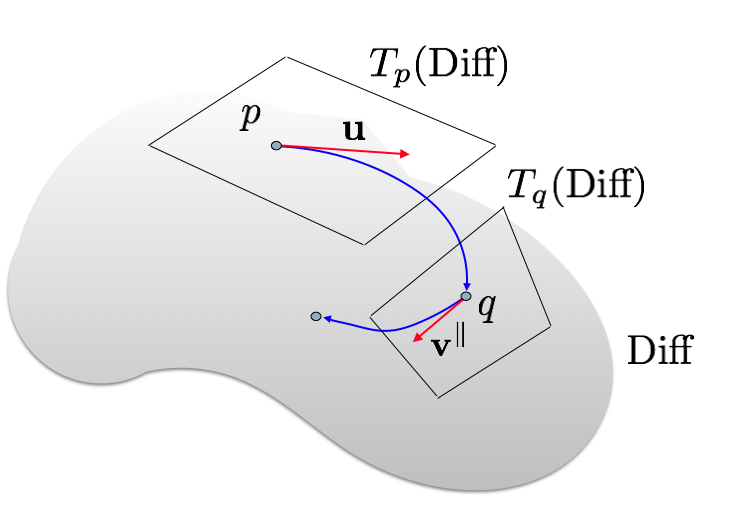
\includegraphics[scale=0.25]{figures/parallel_transport_1.png}
%	\caption{Group composition with offset using parallel transport.}
%	\label{fig:composition}
%\end{figure}
%
%The lack of a close form of any kind and the theoretical difficulties inherent to the investigation of infinite dimensional group of diffeomorphism makes an experimental approach meaningful. 












\part{Tools}\label{pt:tools}

% % % % % % % % % % % % % % % % % % % % % % % % % % % % % % % % % % % % % %
% % % % % % % % % % % % % % % % % % % % % % % % % % % % % % % % % % % % % %
% % SECTION
% % % % % % % % % % % % % % % % % % % % % % % % % % % % % % % % % % % % % %
% % % % % % % % % % % % % % % % % % % % % % % % % % % % % % % % % % % % % %
\chapter{A Lie Group Structure for the Set of Transformation}\label{ch:finite_lie_group}


\begin{flushright}
	\emph{Every working mathematician knows that if one does not control oneself (best of all by examples), then after some ten pages half of all the signs in formulae will be wrong and twos will find their way from denominators into numerators. \\ -V.I. Arnold}
\end{flushright}

%%introductory definition
We consider every group $\mathbb{G}$ as a group of transformation acting on $\mathbb{R}^{d}$, having in mind the particular case $d=2,3$ for 2-dimensional or 3-dimensional images.
We will focus out attention to transformations defined by matrices or diffeomorphism. Other than group they also have the structure of Lie group: they are considered with a maximal atlas that makes them differentiable manifold, in which the composition of two transformation and the inverse of each transformation are well defined differentiable maps:
\begin{align*}
\mathbb{G} \times \mathbb{G} & \longrightarrow  \mathbb{G}    \\
(x,y) &\longmapsto  x y^{-1}
\end{align*}
 Differential geometry is in general a technique to use the well known calculus features and operators on spaces different from the usual $\mathbb{R}^{n}$. Adding the differentiable structure to a group of transformations gives us new handles to hold them: in particular provides the opportunity to define a tangent space to each point of the group (and so a fiber bundle), a space of vector fields, a set of flows and one parameter subgroup as well as other features that enrich this structure. The abstract idea of vector field over a manifold will be concretized for image registration introducing the concepts of \emph{displacement field}, \emph{deformation field} and \emph{velocity field (stationary or time varying)} that will be there presented. Avoid pedantry is as important as to avoid confusions on notations and definitions, therefore it is necessary to call back a few concepts from differential geometry tailored for rigid-body and diffeomorphic image registration, before getting into the heat of the applications. 

% % % % % % % % % % % % % % % % % % % % % % % % % % % % % % % % % % % % % %
% % SUBSECTION
% % % % % % % % % % % % % % % % % % % % % % % % % % % % % % % % % % % % % % 
\section{Velocity Vector Fields and Flows}

Let $\gamma(t)$ be a (continuous) path over a Lie group $\mathbb{G}$, such that $t \in (-\eta,\eta) \subseteq \mathbb{R}$ and $\gamma(0) = p$. If $(C,\psi)$ is a local chart, neighborhood of $p$, the tangent vector of $\gamma$ at the point $p$ can be expressed as
\begin{align*}
\mathbf{u}= \frac{d}{dt}(\psi\circ\gamma)(t) ~\Bigr|_{t=0}
\end{align*}
For different choice of $\gamma$ passing through $p$, we obtain different tangent vectors.
%%%
\[
\begindc{\commdiag}[50]%[50]
\obj(10,10)[G]{$C \subseteq \mathbb{G}$}
\obj(0,0)[R]{$\mathbb{R}$}
\obj(20,0)[Rn]{$\mathbb{R}^{n}$}

\mor{G}{Rn}{$\psi$}
\mor{R}{G}{$\gamma$}
\mor{R}{Rn}{$\psi \circ \gamma$}

\enddc
\]
% 
It can be proved that the set of all of the tangent vector at the point $p$ defines a vector space: the tangent space at $p$, indicated with $T_{p}\mathbb{G}$. It can be proved that this construction do not depend on the local chart's choice. \\
Taking into account the disjoint union of all of the tangent spaces of $\mathbb{G}$ we obtain the tangent bundle $T\mathbb{G}$; it can be proven that it is, in its turn, a differentiable manifold.\\
%% Definition of vector field
Be $\mathbb{G}$ $n$-dimensional Lie group. A \emph{vector field} over $\mathbb{G}$ is a function that assigns at each point $p$ of $\mathbb{G}$, a tangent vector $V_{p}$ in the tangent space $T_{p}\mathbb{G}$, such that $V_{p}$ is differentiable respect to $p$. \\
If $(C; x_{1}, \dots , x_{n}) = (C,\psi)$ is a local chart of $\mathbb{G}$, neighborhood of $p$, then $V_{p}$ can be expressed locally as:
\begin{align*}
V_{p} 
= 
\sum_{i=1}^{n}v_{i}(p) \frac{\partial}{\partial x_{i}}~\Bigr|_{p} 
%=
%v^{i}(p) \partial_{i}\bigr|_{p} 
& & 
v_{i} \in \mathcal{C}^{\infty}(C)
\end{align*}
Using the Einstein summation convention $V_{p}$ is sometime expressed as $V_{p} =  v^{i}(p) \partial_{i}\bigr|_{p} $.
The smooth functions $v_{i}$ define the vector fields in the base 
$(\frac{\partial}{\partial x_{1}}, \dots ,\frac{\partial}{\partial x_{n}})$. The idea of expressing the elements of the base in terms of differential operator reveals the possibility to consider each vector field as a directional derivative over the algebra of smooth functions defined on the manifold.  \\
%% TODO add here an example of the sphere for example! See do carmo vol 1. Do not let more than 5 pages without a concrete example!!
The set of all vector field over $M$, indicated with $\mathcal{V}(M)$, is a real vector space and a module over $\mathcal{C}^{\infty}(M)$:
\begin{align*}
&(V+W)_{p} = V_{p} + W_{p}  &\qquad \forall V, W \in \mathcal{V}(M) \\
&(aV)_{p} = aV_{p} &\qquad \forall a \in \mathbb{R} \\
&(fV)_{p} = f(p)V_{p}  &\qquad \forall V \in \mathcal{V}(M) \quad \forall f \in \mathcal{C}^{\infty}(M)
\end{align*}
Moreover $\mathcal{V}(M)$ acts over $\mathcal{C}^{\infty}(M)$ as follows
\begin{align*}
\mathcal{V}(M) \times \mathcal{C}^{\infty}(M) & \longrightarrow  \mathcal{C}^{\infty}(M) &   \\
(V,f) &\longmapsto  Vf  : \mathcal{C}^{\infty}(M)  \longrightarrow   \mathbb{R} \\
& \qquad \qquad \qquad \quad p \longmapsto (Vf)(p) = V_{p}f
\end{align*}
In the local chart the real number $V_{p}f$ is given by
\begin{align*}
(Vf)(p) = V_{p}f =  \sum_{j=1}^{n}v_{j}(p) \frac{\partial f}{\partial x_{j}}~\Bigr|_{p} 
\end{align*}
and represents the directional derivative of $f$ along the vector $V_{p} \in T_{p}M$.\\
If $(C_{2};y_{1}, \dots , y_{n})$ is another local chart, $p \in C_{2}$, then the change of coordinates can be expressed as follows:
\begin{align*}
V_{p} = \sum_{j=1}^{n} \Big( \sum_{i=1}^{n}v_{i}(p) \frac{\partial y_{j}}{\partial x_{i}}~\Bigr|_{p}  \Big) \frac{\partial }{\partial y_{j}}~\Bigr|_{p}
\end{align*}
A vector field can be time-dependent if each of its vectors varies smoothly within a parameter $t$, otherwise it is time-independent. In this case a continuous function over the set of times $T$ is defined:
\begin{align*}
\mathbb{R} \supseteq T & \longrightarrow  \mathcal{V}(\mathbb{G}) &   \\
t &\longmapsto  V^{(t)}  : \mathbb{G}  \longrightarrow   T\mathbb{G}\\
&  \qquad \qquad \quad p \longmapsto V^{(t)}_{p}
\end{align*}
where $V^{(t)}_{p} $ has local coordinates
\begin{align*}
V^{(t)}_{p} 
=\sum_{i=1}^{n}v_{i}(p,t) \frac{\partial}{\partial x_{i}}~\Bigr|_{p} 
\qquad  
v_{i} \in \mathcal{C}^{\infty}(C\times T)
\end{align*}
Let $V$ a vector field over a differentiable manifold $\mathbb{G}$, an \emph{integral curve} of $V$ is given by
	\begin{align*}
	c : (a,b) & \longrightarrow  \mathbb{G}  \quad \text{such that} \quad 
	\dot{c}(t) = V_{c(t)} \in T_{c(t)}\mathbb{G} ~\forall t\in (a,b)
	\end{align*}
To get the equations of the integral curves, we consider the local expression
\begin{align*}
V
= 
\sum_{i=1}^{n}v_{i} \frac{\partial}{\partial x_{i}} %~\Bigr|_{p} 
%=
%v^{i} \partial_{i} %\bigr|_{p} 
& & 
v_{i} \in \mathcal{C}^{\infty}(C)
\end{align*}
and the unknown curve in the same local chart
\begin{align*}
c(t) = (c_{1}, c_{2}, \dots , c_{n})
\qquad
\dot{c}(t)  = \sum_{i=1}^{n}   \frac{dc_{i}(t)}{dt}   \frac{\partial}{\partial x_{i}} ~\Bigr|_{c(t)} 
\end{align*}
Imposing the condition $\dot{c}(t) = V_{c(t)} $ we get:
\begin{align*}
\sum_{i=1}^{n}   \frac{dc_{i}(t)}{dt}   \frac{\partial}{\partial x_{i}} ~\Bigr|_{c(t)} 
= 
\sum_{i=1}^{n} v_{i}(c(t)) \frac{\partial}{\partial x_{i}} ~\Bigr|_{c(t)}  
\end{align*}
For a given point of the manifold, and considering the integral curves passing for this point we obtain the initial condition $c(0) = p$ for a Cauchy problem :
\begin{equation}
\begin{cases}
\frac{dc_{i}(t)}{dt}  =v_{i}(c_{1}, t_{2}, \dots , c_{n})  \\
c_{i}(0) = p_{i}
\end{cases}
\end{equation}
Thanks to the Cauchy theorem it has a unique solution $\gamma(t)$. The unique integral curve passing through $p$ when $t=0$ is noted by $ c^{(p)}(t)$. \\
Integral curves can be divided in $2$ classes: the one whose domain can be extended to the whole real line $\mathbb{R}$ (in this case $V$ is called \emph{completely integrable vector field}) and the one whose domain is a strict subset of $\mathbb{R}$.
We reminds that the \emph{flow} of the vector field $V$ is the defined as:
\begin{align*}
\Phi_{V}: S\times \mathbb{G} &\longrightarrow \mathbb{G}   \\
(t,p) &\longmapsto  \Phi_{V}(t,p) = c^{(p)}(t)
\end{align*}
where $S = \mathbb{R} $ or $S\subset \mathbb{R}$ if $V$ is or is not respectively completely integrable. Fixing the point $p$, the flow become simply the integral curve passing through $p$; keep $t$ fixed and letting $p$ varying over the manifold, we get the position of each point on the manifold subject to the vector field $V$ at the time $t$. This last idea gives raise to the \emph{one-parameter subgroup}:
\begin{align*}
\forall p \in M \qquad \Phi_{V}(t,p) = \varphi_{t}  \qquad G = \{ \varphi_{t} ~:~ t \in S\}
\end{align*}
\begin{align*}
G\times G &\longrightarrow G   \\
(\varphi_{t_1} ,\varphi_{t_2} ) &\longmapsto  \varphi_{t_1 + t_2} 
\end{align*}
Despite the name, the fact that $G$ forms a group is less important\footnote{In this context: from a group theory point of view the action of the group $(\mathbb{R},+)$ over the manifold has as its orbits, the set of disjoints integral curves.} than considering the compatibility between a sum on the real line and a product between functions. This property will be largely used when dealing with Lie logarithms.
In general a continuous function
\begin{align*}
f : \mathbb{R}\supseteq (-\eta,\eta) & \longrightarrow \mathbb{G}  \qquad f(0) = p
\end{align*}
satisfies the \emph{one parameter subgroup property} if $f(t+s) = f(t) f(s)$ where the last multiplication is the composition on the group. 

% % % % % % % % % % % % % % % % % % % % % % % % % % % % % % % % % % % % % %
% % SUBSECTION
% % % % % % % % % % % % % % % % % % % % % % % % % % % % % % % % % % % % % % 
\section{Push-forward, Left, Right and Adjoint Translation}

Given two Lie group $\mathbb{G}$ and $\mathbb{H}$ linked by the differentiable map $F:\mathbb{G}\rightarrow \mathbb{H}$, then the \emph{push forward} at the point $p$ is defined as the covariant operator
\begin{align*}
(F_{\star})_{p} : T_{p} \mathbb{G} & \longrightarrow  T_{F(p)}\mathbb{H}   \\
V_{p}  &\longmapsto  (F_{\star} V_{p})  : \mathcal{C}^{\infty}(\mathbb{H})  \longrightarrow   \mathbb{R} \\
& \qquad \qquad \qquad \quad f \longmapsto (F_{\star} V_{p})(f) = V_{p}(f\circ F) 
=
v(p)^{i} \partial_{i}(f\circ F)\bigr|_{p} 
\end{align*}
When the point $p$ is implicit by the context it will be omitted: namely $(F_{\star})_{p} = F_{\star}$. \\

In general the push forward gives the right to the vector field $V$ defined over $\mathbb{G}$ to act as a derivative on another manifold $\mathbb{H}$. 
Push forward is well defined since a vector field is completely determined by its action over $\mathcal{C}^{\infty}(\mathbb{H})$.
It can be proved that it is linear, satisfies the Leibnitz rules,  and $(G\circ F )_{\star} = G_{\star} \circ F_{\star}$; moreover, the push forward of the identity is the identity map between vector spaces, and if $F$ is a diffeomorphism, $F_{\star}$ is an isomorphism of vector spaces. \\
The \emph{pull-back}, is defined on the dual space of $\mathbb{G}$ and $\mathbb{H}$ as the contravariant operator of the push forward\footnote{Push-forward is defined between vector spaces, pull-back between space of functions and $V_{p}(F^{\star} f ) =  (v(p)^{i} \partial_{i}\bigr|_{p} )(f\circ F) = v(p)^{i} \partial_{i}(f\circ F)\bigr|_{p} = V_{p}(f\circ F) $.}:
\begin{align*}
F^{\star} : \mathcal{C}^{\infty}(\mathbb{H}) & \longrightarrow  \mathcal{C}^{\infty}(\mathbb{G})    \\
f  &\longmapsto  F^{\star} f  := f\circ F
\end{align*}
The following diagram relates pull-back and push-forward:
\[
\begindc{\commdiag}[29]
\obj(-30,30)[TM]{$T_{p}\mathbb{G}$}
\obj(0,30)[TN]{$T_{p}\mathbb{H}$}

\obj(-30,10)[M]{$\mathbb{G}$}
\obj(0,10)[N]{$\mathbb{H}$}
\obj(30,10)[R]{$\mathbb{R}$}

\mor{TM}{TN}{$F_{\star}$}

\mor{M}{N}{$F$}
\mor{N}{R}{$f$}

\mor{TM}{M}{}[1, 1]
\mor{TN}{N}{}[1, 1]

\cmor((-30,6)(-29,4)(-25,3)(0,3)(25,3)(29,4)(30,6)) 
\pup(0,0){$F^{\star}f$}


\enddc
\]

\noindent
Here we restrict our attention at the case $\mathbb{G}=\mathbb{H}$, thus $F$ is a map that moves the points of $\mathbb{G}$ smoothly.
Each element $p$ of a Lie group $\mathbb{G}$ defines three maps on $\mathbb{G}$:
\begin{enumerate}
	\item \emph{left-translation}:
		\begin{align*}
		L_{p}: \mathbb{G} & \longrightarrow  \mathbb{G} \\
		q &\longmapsto pq
		\end{align*}
	\item \emph{right-translation}:
			\begin{align*}
			R_{p}: \mathbb{G} & \longrightarrow  \mathbb{G}\\
			q &\longmapsto qp
			\end{align*}
	\item \emph{adjoint map} 
			\begin{align*}
			\text{Ad}_{p}: \mathbb{G} & \longrightarrow  \mathbb{G} \\
			q &\longmapsto pqp^{-1}
			\end{align*}
\end{enumerate}
The push forward for the vector field $V$ at the point $q$ are given by:
\begin{enumerate}
	\item \emph{left-translation}:
	\begin{align*}
	(L_{p})_{\star}V_{q}f 
	=
	V_{q}(f\circ L_{p}) 
	=
	\sum_{i=1}^{n} v_{i}(q) \frac{\partial f \circ L_{p}}{\partial x_{i}} ~\Bigr|_{q} 
	=   
	\sum_{i=1}^{n} v_{i}(q) \frac{\partial f }{\partial x_{i}} ~\Bigr|_{pq} 
	\end{align*}
	\item \emph{right-translation}:
	\begin{align*}
	(R_{p})_{\star}V_{q}f 
	=
	V_{q}(f\circ R_{p}) 
	=
	\sum_{i=1}^{n} v_{i}(q) \frac{\partial f \circ R_{p}}{\partial x_{i}} ~\Bigr|_{q} 
	=   
	\sum_{i=1}^{n} v_{i}(q) \frac{\partial f }{\partial x_{i}} ~\Bigr|_{qp} 
	\end{align*}
	\item \emph{adjoint map} 
	\begin{align*}
	(\text{Ad}_{p})_{\star}V_{q}f 
	=
	V_{q}(f\circ \text{Ad}_{p}) 
	=
	\sum_{i=1}^{n} v_{i}(q) \frac{\partial f \circ \text{Ad}_{p}}{\partial x_{i}} ~\Bigr|_{q} 
	=   
	\sum_{i=1}^{n} v_{i}(q) \frac{\partial f }{\partial x_{i}} ~\Bigr|_{pqp^{-1}} 
	\end{align*}
\end{enumerate}
We note that in each expression the coefficient $v_{i}(q)$ remains the same even if the partial derivative is not applied at the point $q$. Therefore the linear combination of the constant coefficients $v_{i}(q)$ can be considered as a scalar product with the elements of the base applied at the function $f$.
Left and right translation of the vector $\mathbf{u}$ can be expressed as scalar product with the \emph{differential}, equivalent concept as the push forward, that emphasizes the scalar product implied in the definition:
\begin{align*}
(DL_{p})_{q} : T_{q} \mathbb{G}& \longrightarrow  T_{pq}\mathbb{G}    \\
\mathbf{u} &\longmapsto  (DL_{p})_{q} \cdot \mathbf{u} 
\end{align*}
\begin{align*}
(DR_{p})_{q} : T_{q} \mathbb{G} & \longrightarrow  T_{qp}\mathbb{G}    \\
\mathbf{u} &\longmapsto  (DR_{p})_{q} \cdot \mathbf{u}
\end{align*}
where $(DL_{p})_{q}$, $(DR_{p})_{q}$ are properly defined vectors that can be expressed local coordinates as follow
\begin{align*}
(DL_{p})_{q} = \sum_{i=1}^{n}\frac{\partial }{\partial x_{i}} ~\Bigr|_{pq}
\qquad 
(DR_{p})_{q} = \sum_{i=1}^{n} \frac{\partial }{\partial x_{i}} ~\Bigr|_{qp}
\end{align*}
Or equivalently linear operators defined as:
\begin{align*}
(DL_{p})_{q} : \mathcal{C}^{\infty}(M) & \longrightarrow  \mathbb{R}   \\
 f &\longmapsto  (DL_{p})_{q} (f) = \frac{\partial f}{\partial x_{i}} ~\Bigr|_{pq} 
 \end{align*}
 \begin{align*}
(DR_{p})_{q} : \mathcal{C}^{\infty}(M) & \longrightarrow  \mathbb{R} \\
f &\longmapsto  (DR_{p})_{q} (f) = \frac{\partial f}{\partial x_{i}} ~\Bigr|_{qp}
\end{align*}
A change of notation $V_{q} = \mathbf{u}$ makes push-forward and differential strikingly equivalent. This holds also for the generic map F:
\begin{align*}
(DF)_{q} (f)= \sum_{i=1}^{n}\frac{\partial f\circ F}{\partial x_{i}} ~\Bigr|_{q}
\qquad
(DF)_{q} (f)\cdot \mathbf{u}  = \sum_{i=1}^{n} u_{i}\frac{\partial f\circ F}{\partial x_{i}} ~\Bigr|_{q}
\end{align*}
The subscript $q$ in $(DL_{p})_{q}$ can be omitted when the tangent space of $\mathbf{u}$ is clear by the context. 

%------------------ definition of left invariant vector field
A vector field $V$ defined over a manifold is \emph{left-invariant} if it is invariant for each left translation. It means that $(L_{q})_{\star} V_{p} = V_{p}$ for any choice of $p$ and $q$. If we consider all of the possible push forward of the left translation applied to a single tangent vector at the origin $\mathbf{v}$ of $T_{e}\mathbb{M}$ we have a unique left-invariant vector field defined as $\mathbf{v}^{L}$ such that
\begin{align*}
\mathbf{v}^{L}_{q} := (L_{q})_{\star} \mathbf{v} \qquad \forall q \in M
\end{align*}
Vice versa every left-invariant vector field $V$ is uniquely represented by $V_{e}$.
 The set of all of the left-invariant vector fields form a linear subspace of the space of the vector field, indicated with $\text{left}\mathcal{V}(M)$. This can be easily proved by:
\begin{align*}
(L_{g})_{\star} (aV +bW) = a (L_{g})_{\star} V + b (L_{g})_{\star} W
\qquad 
\forall V, W \in \mathcal{V}(\mathbb{G}) 
\quad 
\forall a, b \in \mathbb{R}
\end{align*}
In fact for each $h \in \mathbb{G}$ and for each $f \in \mathcal{C}^{\infty}(\mathbb{G})$ the linearity property holds:
\begin{align*}
(L_{g})_{\star} (aV_{h} +bW_{h})f &= (aV_{h} +bW_{h})(f\circ L_{g} ) \\
&= aV_{h}(f\circ L_{g} ) +bW_{h}(f\circ L_{g} ) \\
&= a (L_{g})_{\star} V_{h}f + b (L_{g})_{\star} W_{h}f  
\end{align*}
The linearity property leads to the definition of the group of homomorphism over $\mathbb{G}$. It is the set of all the Lie group homomorphism from $\mathbb{R}$ to $\mathbb{G}$:
\begin{align*}
Hom(\mathbb{R},\mathbb{G}) = \lbrace \varphi: \mathbb{R} \rightarrow \mathbb{G} \mid \varphi(a+b) = \varphi(a) \circ \varphi(b)\phantom{aa} \forall a,b \in \mathbb{R} \rbrace
\end{align*}
Tangent spaces, flows, one-parameter subgroup and Lie group homomorphisms are bounded together by the following remarkable result, which is a most important precondition for the definition of the Lie group exponential, and so deserve to be written in form of a lemma and formally proved. 
\begin{lemma}
	Let $\mathbb{G}$ be a Lie group. For each $\mathbf{v}$ in the tangent space $T_{e}\mathbb{G}$, exists a unique homomorphism $\gamma_{\mathbf{v}}$ in $Hom(\mathbb{R},\mathbb{G})$ (or equivalently a function satisfying the one-parameter subgroup property) such that 
	\begin{align*}
	\dot{\gamma}_{\mathbf{v}}(0) = \mathbf{v}
	\end{align*}
\end{lemma}
\begin{proof}
	The homomorphism $\gamma_{\mathbf{v}}$ coincides with the integral curve $\Phi$ of the left invariant vector field generated by $\mathbf{v}$ passing through the identity. Its uniqueness is then a consequence of the Cauchy theorem. The same theorem also specifies the existence for a small enough neighbour $(-\eta,\eta)\subset \mathbb{R}$. To extend the solution to the whole $\mathbb{R}$ it is enough to consider that $\gamma_{\mathbf{v}}(t+s) = \gamma_{\mathbf{v}}(t) \gamma_{\mathbf{v}}(s)$ for each $s,t \in (-\eta,\eta)$:
	\begin{align*}
	\gamma_{\mathbf{v}}(t+s) = \Phi(t+s,e) =\Phi(t,\gamma_{\mathbf{v}}(s)) = \gamma_{\mathbf{v}}(t) \gamma_{\mathbf{v}}(s)
	\end{align*}
	%completeness missing, should refer to a subset of the real line instead the whole real line!
\end{proof}
We observe that $\gamma_{\mathbf{v}}$ is exactly the one parameter subgroup of $\mathbf{v}^{L}$ defined above, and then we can write $\gamma_{\mathbf{v}}(t) = \Phi(t,e) = \varphi_{e}(t)$.\\

We conclude this paragraph remembering the definition of the Lie algebra of a Lie group that take into account every feature so far introduced:
\begin{definition}
	Given a Lie group $\mathbb{G}$, its Lie algebra $\mathfrak{g}$ is defined as:
	\begin{enumerate}
		\item The vector space $T_{e}\mathbb{G}$  of all of the tangent vector at the identity (or at any other point of the manifold): $\mathfrak{g} := T_{e}\mathbb{G}$.
		\item The set of the left invariant vector Field over $\mathbb{G}$: $\mathfrak{g} := \text{left}\mathcal{V}(\mathbb{G})$.
		\item The set of all of the flows passing through $e$:  $\mathfrak{g} := \{ \Phi(e,t) : t \in S\subseteq \mathbb{R} \}$.
		\item The set of homomorphism $Hom(\mathbb{R},\mathbb{G}) $.
	\end{enumerate}
\end{definition}
The Lie algebra can be also defined independently from a Lie group as a vector space endowed with Lie bracket (bilinear form, antisymmetric, that satisfies the Jacobi identity). In the finite dimensional case given a Lie algebra $\mathfrak{g}$ it can be proved that exists always a Lie group $\mathbb{G}$ such that $\mathfrak{g}$ is the Lie algebra defined over $\mathbb{G}$. This property (third Lie theorem) do not holds anymore infinite dimensional Lie algebra of diffeomorphisms.

% % % % % % % % % % % % % % % % % % % % % % % % % % % % % % % % % % % % % %
% % SUBSECTION
% % % % % % % % % % % % % % % % % % % % % % % % % % % % % % % % % % % % % % 
\section{Lie Exponential, Lie logarithm and the Log-composition}
Let $\mathbf{v}$ be an element in the tangent space $\mathfrak{g}$ and $V\in\text{left}\mathcal{V}(\mathbb{G})$ the unique vector field defined by $\mathbf{v}$ over a local coordinate system around the origin. Let $\Phi$ be the flow associated with the vector field and $\gamma(t)$ the unique integral curve of $v$ passing through the identity of the group.  
The \emph{Lie exponential} is defined as
\begin{align*}
\exp :  \mathfrak{g} & \longrightarrow  \mathbb{G}  \\
\mathbf{v} &\longmapsto  \exp(\mathbf{v} ) = \gamma(1)
\end{align*}
It satisfies the following properties:
\begin{enumerate}

	 	\item $\exp(V) = e$ if $V = 0$.
	 	\item $\exp(V)$ is invertible and $(\exp(V))^{-1} = \exp(-V)$.
	 	\item $\exp((a+b)V) = \exp(aV)\exp(bV)$.
	 	\item If $U$ and $V$ are commutative then $\exp(V + U) = \exp(V)\exp(U)$.
	 	%\item If $C$ is an invertible element in then $\exp(CVC^{-1}) = C\exp(V)C^{-1}$.
	 	\item For any norm $\euclideanMetric{\exp(V)} \leq \exp(\euclideanMetric{V})$.

\end{enumerate}
The inverse of the Lie $\exp$ is defined by
\begin{align*}
\log : \mathbb{G} & \longrightarrow \mathfrak{g} \\
p &\longmapsto \log (p)  =  \mathbf{v}   
\end{align*}
where $\mathbf{v}  $ is the tangent vector having $p$ as it $\exp$.
The following properties holds:
\begin{enumerate}
	\item ....
\end{enumerate} 


% % % % % % % % % % % % % % % % % % % % % % % % % % % % % % % % % % % % % %
% % SUBSECTION
% % % % % % % % % % % % % % % % % % % % % % % % % % % % % % % % % % % % % % 
\section{BCH formula for the Computation of Log-composition}



Let $\mathbf{u},\mathbf{v}$ be element of the Lie algebra. The solution $\mathbf{w}$ of the equation $exp(\mathbf{w}) = \exp(\mathbf{u}) \circ \exp(\mathbf{v})$ is provided by the BCH formula, when $\bf{v}$ is small:
\begin{align*}
BCH(\mathbf{u},\mathbf{v}) 
= 
\mathbf{u} + \mathbf{v} + \frac{1}{2}[\mathbf{u},\mathbf{v}] + \frac{1}{12}([\mathbf{u},[\mathbf{u},\mathbf{v}]]
+ [\mathbf{v},[\mathbf{v},\mathbf{u}]]) - \frac{1}{24}[\mathbf{v},[\mathbf{u},[\mathbf{u},\mathbf{v}]]] +... 
\end{align*}

....Nested Lie bracket can be written using multiple composition of the \emph{adjoint action} of $\mathbf{u}$ on the Lia algebra:
\begin{align*}
ad_{\mathbf{u}} : \mathfrak{g}  & \longrightarrow \mathfrak{g}  
\\
\mathbf{v} &\longmapsto ad_{\mathbf{u}}   =  [\mathbf{u}, \mathbf{v}]
\end{align*}
With this operator we can write 
\begin{align*}
[  \underbrace{   \mathbf{u},[\mathbf{u},... [\mathbf{u}}_{\text{n-times}},\mathbf{v}]...]] =  ad_{\mathbf{u}}^{n}(\mathbf{v})
\end{align*}
In the appendix of ....Klarsfeld adjoint action are used to provide an expansion of the BCH formula. This can be rewritten as
\begin{align*}
BCH(\mathbf{u},\mathbf{v})  = \mathbf{u} + \frac{ ad_{\mathbf{u}} \exp(ad_{\mathbf{u}}) }{ \exp(ad_{\mathbf{u}}) - 1 }  \mathbf{v} + O({\mathbf{v}}^2)
\end{align*}
The functional applied to $\mathbf{v}$ can be rewritten as
\begin{align*}
\frac{ ad_{\mathbf{u}} \exp(ad_{\mathbf{u}}) }{ \exp(ad_{\mathbf{u}}) - 1 }  = \sum_{n=0}^{\infty} \frac{B_{n}}{n!} ad_{\mathbf{u}}^{n} 
\end{align*}
Where $\lbrace B_{n} \rbrace $ is the sequence of the second-kind Bernoulli number\footnote{If first-kind Bernoulli number is used then each term of the summation must be multiplied for $(-1)^{n}$, as did for example in ....Klarsfeld.}.

% % % % % % % % % % % % % % % % % % % % % % % % % % % % % % % % % % % % % %
% % SUBSECTION
% % % % % % % % % % % % % % % % % % % % % % % % % % % % % % % % % % % % % % 
\section{Taylor Expansion for the Computation of Log-composition}




\chapter{Parallel Transport Tool}\label{ch:parallel_transport}

In this section we present parallel transport for the finite dimensional Lie group and we make the assumption that obtained results hold in the infinite dimensional case.




% % % % % % % % % % % % % % % % % % % % % % % % % % % % % % % % % % % % % %
% % SUBSECTION
% % % % % % % % % % % % % % % % % % % % % % % % % % % % % % % % % % % % % % 
\section{Connections and Geodesics}

.... definition of connection and geodesics. Properties that concern us.

% % % % % % % % % % % % % % % % % % % % % % % % % % % % % % % % % % % % % %
% % SUBSECTION
% % % % % % % % % % % % % % % % % % % % % % % % % % % % % % % % % % % % % % 
\section{Affine $\exp$ and Affine $\log$}
Any Lie group $\mathbb{G}$ considered with a left-invariant connection $\nabla$ can be equipped with a metric based on the elements of its tangent space:
\begin{align*} 
	\text{dist}(x,y) := \euclideanMetric{\log_{e}(x^{-1}\circ y) } \qquad \forall x, y \in \mathbb{G}
\end{align*}
Where the $\log$ function is the \emph{Affine logarithm}, inverse function of the the \emph{Affine exponential}:
\begin{align*}
	\log : \mathbb{G} \times  \mathbb{G}  & \longrightarrow T \mathbb{G}  
	\qquad \qquad \quad \quad 
	\exp : \mathbb{G} \times T \mathbb{G}     \longrightarrow T \mathbb{G}  
	\\
	(p,q) &\longmapsto \log _{p}(q)  =  V_{p}  
	\qquad \qquad \quad   
	(p,q) \longmapsto \exp _{p}(q)  =  \gamma(1)
\end{align*}
for $V$ is the tangent vector field of the geodesic $\gamma$ drawn on $\mathbb{G}$, passing through $p$ and $q$, 
\begin{align*}
	\gamma(0) = p, ~~ \gamma(1)=q, ~~\nabla_{\dot{\gamma}}\dot{\gamma} = 0
\end{align*}
and having $V_{p}$ as its tangent vector at $p$:
\begin{align*}
	\log _{p}(q)   = V ~&\Leftrightarrow ~ V_{\gamma(t)} = \dot{\gamma}(t) ~~ \forall t \in [0,1]\\
	\exp _{p}(q)  =  \gamma(1) ~&\Leftrightarrow ~ \dot{\gamma}(p) = V_{p}
\end{align*}
The left-invariant condition over $\nabla$ has some consequences: 
\begin{enumerate}
	\item the vector field $V$ resulting by the application of the $\log$ function is left-invariant, so it is an element of the Lie algebra $\mathfrak{g}$ and uniquely determined by $V_{\text{e}}$. 
	\item Affine $\exp$ and $\log$ and coincides with Lie $\exp$ and $\log$.
	\item $V$ is a complete vector field.
\end{enumerate}	


% % % % % % % % % % % % % % % % % % % % % % % % % % % % % % % % % % % % % %
% % SUBSECTION
% % % % % % % % % % % % % % % % % % % % % % % % % % % % % % % % % % % % % % 
\section{Parallel Transport through Examples}
\begin{definition}
	Let $\mathbb{G}$ be a finite dimensional connected Lie group defined with a connection $\nabla$. Given $a,b \in \mathbb{G}$ and $\gamma : [0,1] \rightarrow \mathbb{G}$ such that $\gamma(0) = a$ and $\gamma(1) = b$, then the vector $X_{a} \in T_{a}\mathbb{G}$, belonging to some vector field $X$ is parallel transported along $\gamma$ up to $T_{b}\mathbb{G}$ if for all $t \in  [0,1]$ $\nabla_{\dot{\gamma}}X_{\gamma(t)} = 0$.\\
	The parallel transport is the function that maps $X_{a}$ from $T_{a}\mathbb{G}$ to $T_{b}\mathbb{G}$ along $\gamma$:
	\begin{align*}
		\Pi(\gamma)_{a}^{b} :  T_{p}\mathbb{G} & \longrightarrow T_{b}\mathbb{G}  \\
		X_{a}&\longmapsto \Pi(\gamma)_{a}^{b}(X_{p}) = Y_{b}
	\end{align*}
\end{definition}


\begin{theorem}[Inversion]
	$\mathbb{G}$ Lie group, $\nabla$ connection, $a,b\in\mathbb{G}$. Given $\gamma$ such that $\gamma(0)= a$, $\gamma(1)=b$ and $\dot{\gamma}(0)=\mathbf{u}\in T_{a}\mathbb{G}$, we have:
	\begin{align}
		\Pi(\gamma)_{a}^{b}(-\mathbf{u}) &= -\Pi(\gamma)_{a}^{b}(\mathbf{u}) \\
		a = \exp_{b}(\mathbf{u}) \Longleftrightarrow& \phantom{z} b = \exp_{a}(-\Pi(\gamma)_{b}^{a}(\mathbf{u}))
	\end{align}
\end{theorem}
How does the change of sign behave when the Lie group exponential is expressed as a composition is explored in the next property:
\begin{theorem}[Inversion for composition, Lie exponential]
	$\mathbb{G}$ Lie group, $\mathbf{u}, \mathbf{v}, \mathbf{w}\in T_{e}\mathbb{G}$. If
	\begin{align*}
		\exp(\mathbf{w}) = \exp(\mathbf{u}) \circ \exp(\mathbf{v})
	\end{align*}
	then
	\begin{align*}
		\exp(\mathbf{-w}) = \exp(\mathbf{-v}) \circ \exp(\mathbf{-u})
	\end{align*}
\end{theorem}
In the next property we explore how does behave the affine exponential expressed as a composition when changed of sign:
\begin{theorem}[Inversion for composition, affine exponential]
	$\mathbb{G}$ Lie group, $\nabla$ connection, $a,b\in\mathbb{G}$, $\mathbf{u}\in T_{a}\mathbb{G}$, $\mathbf{v}\in T_{b}\mathbb{G}$. Let $\beta$ be the tangent curve to $\mathbf{u}$ at $a$ and $c= \exp_{b}(\mathbf{v})$. Given $\mathbf{w} \in T_{c}\mathbb{G}$ such that 
	\begin{align*}
		\exp_{a}(\mathbf{w}) = \exp_{b}(\mathbf{v}) \circ \exp_{a}(\mathbf{u})
	\end{align*}
	Then
	\begin{align*}
		\exp_{a}(-\mathbf{w}) = \exp_{\tilde{b}}(-\Pi(\beta)_{b}^{\tilde{b}}(\mathbf{v})) \circ \exp_{a}(-\mathbf{u})
	\end{align*}
	where $\tilde{b}$ is the affine exponential of $-\mathbf{u}$ or the element $\beta(-1)$.
\end{theorem}

% % % % % % % % % % % % % % % % % % % % % % % % % % % % % % % % % % % % % %
% % SUBSECTION
% % % % % % % % % % % % % % % % % % % % % % % % % % % % % % % % % % % % % % 
\section{Change of Base Formulas with and without Parallel Transport}
Using the derivative of the left-translation $L_{p}$ it is possible to bring back the $\exp$ and the $\log$ function based at the point $p$ of the manifold to the one evaluated at the identity using the following formulas:
\begin{align*}
	\log _{p}(q)  &= DL_{p}(e) \log _{e}(q)  \\
	\exp _{p}(\mathbf{u})  &= p\circ \exp_{e} (DL_{p}(e)^{-1} \mathbf{u})
\end{align*}
....Proof and examples..


% % % % % % % % % % % % % % % % % % % % % % % % % % % % % % % % % % % % % %
% % SUBSECTION
% % % % % % % % % % % % % % % % % % % % % % % % % % % % % % % % % % % % % % 
\section{Parallel Transport in Practice: Schild's Ladder and Pole Ladder}

....
% % % % % % % % % % % % % % % % % % % % % % % % % % % % % % % % % % % % % %
% % % % % % % % % % % % % % % % % % % % % % % % % % % % % % % % % % % % % %
% % SECTION
% % % % % % % % % % % % % % % % % % % % % % % % % % % % % % % % % % % % % %
% % % % % % % % % % % % % % % % % % % % % % % % % % % % % % % % % % % % % %

\chapter{Accelerating Convergences Series}\label{ch:accelerating}

xxx Think about it after 14 of may!

Space of the series of elements of $\mathfrak{g}$
\begin{align*}
S(\mathfrak{g}) = \{ \sum_{j=0}^{\infty} \mathbf{u}_{j} \mid \mathbf{u}_{j} \in \mathfrak{g}  \}
\end{align*}
Series generate by 
\begin{align*}
S(\mathbf{u}) =\sum_{j=0}^{\infty} \mathbf{u}^{j} 
\end{align*}
\begin{align*}
\exp(\mathbf{u}) = S_1  \cdot S(\mathbf{u}) 
\end{align*}
where $S_1 = \sum_{k=0}^{\infty} (\frac{1}{k!})$ in the space of coefficient series $\cdot $ is the (infinite) scalar product in the space of series.\\
$k$-th series truncation:
\begin{align*}
S^{k}(\mathfrak{g})  = \{ \sum_{j=0}^{k} \mathbf{u}_{j} \mid \mathbf{u}_{j} \in \mathfrak{g}  \}
\end{align*}
This notation may make sense as a starting point to define $\exp(\mathbf{u})$. 
The restriction to the first order truncation of the exp is the starting point the numerical approximation
\begin{align*}
\exp(\mathbf{u}) = 1 + \mathbf{u} \in S^{1}(\mathfrak{g}) 
\end{align*}
\part{Studied Objects}\label{pt:studied_objects}

\chapter{The Group of Rigid Body Transformations}\label{ch:rigid_body_transformations}

\begin{flushright}
	\emph{People know or dimly perceive, that if thinking is not kept pure and keen, if spirit's contemplation do not holds, even mechanics of automobiles and ships will soon cease to run. Even engineer's slide rule, computations of banks and stock exchanges will wonder aimlessly for the lost of authority, and chaos will ensue.} \\ -Hermann Hesse, \emph{Magister Ludi}
\end{flushright}


A rigid body transformation in a normed vector space is a transformation that preserves distances. The set of rigid body transformations is constructed as any combination of rotations, translations and reflection. We are interested in two things about them: their expression in matrix form, and the Lie group structure they form. In particular we will develop the close formulas for the computation of the log composition, and for each approximation technique presented. In part \ref{pt:applications}, they will be compared with the same technique applied to SVF where no ground truth is known.

\section{Lie Logarithm and Exponential for SE(2)}

The set of all of the $3\times 3$  matrices with real entries is denoted with $M_{3}(\mathbb{R})$. 
Its subset, defined by all the matrices with non-zero determinant, and thus by all the invertible matrices, is denoted with $GL_3 (\mathbb{R})$. A matrix group is any subgroup of  $GL_3 (\mathbb{R})$.
We are interested in writing the group of rigid body transformation 
\begin{align*}
\mathbb{G} =
\{ (\theta, tx, ty) \mid \theta \in [0, 2\pi),   tx, ty \in\mathbf{R}^2  \}
\end{align*}
using matrices, so as a subgroup of $GL_3 (\mathbb{R})$.
Rotation in the plane can be expressed using matrix of the orthogonal group $SO(2)$, linear subgroup of $GL_2 (\mathbb{R})$, so that rotations' actions on planes' points are simply defined as a product: 
\begin{align*}
SO(2) = 
\left \{
\left (
\begin{array} {c c }
\cos(\theta) & - \sin(\theta) \\
\sin(\theta) & \cos(\theta) 
\end{array}
\right )
\mid
\theta \in  [0, 2\pi)
\right \}
\end{align*}
To include the translation we can add its $(tx, ty)^{T}$ parameter to the action of the rotation over the initial point $(x_{i}, y_{i})^{T}$ to obtain the transformed $(x_{t}, y_{t})^{T}$. So each element of the group $\mathbb{G}$ act over $\mathbf{R}^2$ as
\begin{align*}
\left (  
\begin{array} {c }
x_{t} \\
y_{t}
\end{array}
 \right ) 
 = 
\left (
\begin{array} {c c }
\cos(\theta) & - \sin(\theta) \\
\sin(\theta) & \cos(\theta) 
\end{array}
\right )
\left (  
\begin{array} {c }
x_{i} \\
y_{i}
\end{array}
\right ) 
+
\left (  
\begin{array} {c }
tx \\
ty
\end{array}
\right ) 
\end{align*}
Another way to express rigid body transformation group's elements is to include the translation in a bigger matrix, subgroup (not linear, since the translation is not linear) of $GL_3 (\mathbb{R})$. This is defined as the group $SE(2)$:
\begin{align*}
SE(2) = 
\left \{
\left (
\begin{array} {c c c }
\cos(\theta) & - \sin(\theta)& t_{x} \\
\sin(\theta) & \cos(\theta) & t_{y}\\
0 & 0 &  1
\end{array}
\right )
\mid
\theta \in  [0, 2\pi), (tx, ty) \in\mathbf{R}^2
\right \}
\end{align*}
Expressed in this way the matrices act on the point of the plane represented as the elements of the vector space $\{1 \} \times \mathbf{R}^2$.\\ 
The passage between the restricted form $\mathbb{G} $ and $SE(2)$ is defined by the injection:
\begin{align*}
\rho_{\mathbb{G}} : \mathbb{G} &\longrightarrow   SE(2)\\
(\theta, tx, ty) 
& \longmapsto
\left (
\begin{array} {c c c }
\cos(\theta) & - \sin(\theta)& tx \\
\sin(\theta) & \cos(\theta) & ty\\
0 & 0 &  1
\end{array}
\right )
\end{align*}
We are now interested the Lie algebra of the Lie group $SE(2)$. 
%In general a matrix Lie group is any complete subgroup of $GL(n,\mathbb{R})$ while its Lie algebra is a particular subset (not necessarily a group) of $GL(n,\mathbb{R})$. 
%\begin{prop}\label{pr:matrixLiealgebra}
%	Be $\mathbb{G}$ a matrix Lie group.
%	\begin{itemize}
%		\item[a)] If $\mathbb{G} = GL(n,\mathbb{R})$ then $T_{e}\mathbb{G} = M(n,\mathbb{R})$.  
%		\item[b)] If $\mathbb{G} \subseteq GL(n,\mathbb{R})$ then $T_{e}\mathbb{G} \subseteq M(n,\mathbb{R})$.
%	\end{itemize}
%\end{prop}
%\begin{proof}
%	since $det$ is a continuous function we have that 
%	\begin{align*}
%	\forall X \in M(n,\mathbb{R})~~ \exists &\eta > 0 \text{ such that } \forall t \in(-\eta , \eta) \\
%	&det(I+tX) \neq 0
%	\end{align*}
%	where $I$ is the identity matrix. If we consider the path
%	\begin{align*}
%	\gamma : [0,1] & \longrightarrow  GL(n,\mathbb{R}) \\
%	t &\longmapsto I+tX
%	\end{align*}
%	as the path joining $I$ and $X$, it follows
%	\begin{align*}
%	\frac{d }{dt}(I+tX)~\Bigr|_{t = 0}  = X \in M(n,\mathbb{R})
%	\end{align*}
%\end{proof}
It is defined as:
\begin{align*}
	\mathfrak{se}(2) = 
	\left \{
	\left (
	\begin{array} {c c c }
		0 & -\theta &  dt_{x} \\
		\theta & 0 & dt_{y} \\
		0& 0 & 1
	\end{array}
	\right )
	\mid
	\theta \in  [0, 2\pi), (tx, ty) \in\mathbf{R}^2
	\right \}
\end{align*}
Expressing $r\in SE(2)$ as:
\begin{align*}
\mathbf{r} = 
\left (
\begin{array} {c c }
R(\theta) & t \\
0 & 1 
\end{array}
\right )
\qquad
R(\theta) \in SO(2) 
\quad
t \in \mathbb{R}^{2}
\end{align*}
for $t$ plane translation and $R(\theta)$ in $SO(2)$, then the element of the Lie algebra can be expressed as:
\begin{align*}
d\mathbf{r} 
= 
\left (
\begin{array} {c c }
dR(\theta) & dt \\
0 & 1 
\end{array}
\right )
\qquad
R(\theta) \in SO(2) 
\quad
t \in \mathbb{R}^{2}
\end{align*}
Both $SE(2)$ and $\mathfrak{se}(2)$ are in bijective correspondence with $\mathbb{G}$, and both are subset of the bigger algebra of, The algebra $\mathfrak{se}(2)$ do not form a group with the operation of composition, but it is provided with the lie bracket defined by the commutator:
\begin{align*}
[d\mathbf{r}, d\mathbf{s}] = d\mathbf{r} d\mathbf{s} - d\mathbf{s} d\mathbf{r}
\end{align*}
The Lie logarithm between Lie group and Lie algebra is given by:
\begin{align*}
\log : \mathfrak{se}(2) & \longrightarrow SE(2)
\\
\left (
\begin{array} {c c }
R(\theta) & t \\
0 & 1 
\end{array}
\right )
&\longmapsto  
\left (
\begin{array} {c c }
dR(\theta) & dt \\
0 & 1 
\end{array}
\right )
\end{align*}
Where 
\begin{align*}
dR(\theta) = 
\left (
\begin{array} {c c }
 0 & -\theta \\
\theta & 0 
\end{array}
\right )
\end{align*}
and $dt = L(\theta)t$ for 
\begin{align*}
L(\theta) = 
\frac{\theta}{2}
\left (
\begin{array} {c c }
\frac{\sin(\theta)}{1-\cos(\theta)} & 1 \\
-1 & \frac{\sin(\theta)}{1-\cos(\theta)}
\end{array}
\right )
\end{align*}
The inverse function, Lie exponential is given by:
\begin{align*}
\exp : SE(2) & \longrightarrow \mathfrak{se}(2) 
\\
\left (
\begin{array} {c c }
dR(\theta) & dt \\
0 & 1 
\end{array}
\right )
&\longmapsto  
\left (
\begin{array} {c c }
R(\theta) & t \\
0 & 1 
\end{array}
\right )
\end{align*}
 where $t = L(\theta)^{-1}dt$ for 
 \begin{align*}
 L(\theta)^{-1} = 
 \frac{1}{\theta}
 \left (
 \begin{array} {c c }
 \sin(\theta) & -(1-\cos(\theta)) \\
 (1-\cos(\theta)) & \sin(\theta)
 \end{array}
 \right )
 \end{align*}
The proposed exponential function is not well defined over all $\mathfrak{se}(2)$.\\
In fact the elements of $\mathbb{G}$ can be identified with no risk with their matrices, while the same thing do not happen for the element of the Lie algebra $\mathfrak{g}$ of $\mathbb{G}$. 
If we formalize the passage between $\mathfrak{g} $ and $\mathfrak{se}(2)$ with the function:
\begin{align*}
\rho_{\mathfrak{g}} : \mathfrak{g} &\longrightarrow  \mathfrak{se}(2)\\
(\theta, dtx, dty) 
& \longmapsto
\left (
\begin{array} {c c c }
0 & -\theta & dtx \\
\theta & 0 & dty\\
0 & 0 &  1
\end{array}
\right )
\end{align*}
it is not an injection if we do not restrict its domain. In addition, given two elements $(\theta_{0}, dtx_{0}, dty_{0})$ and $(\theta_{1}, dtx_{1}, dt_{1})$ in $\mathfrak{g}$, with $\theta_{1}\neq 0$, we have that for each $k\in \mathbb{Z}$, if
\begin{align*}
\theta_{0} = \theta_{1} + 2k\pi
\end{align*}
and
\begin{align*}
(dtx_{0}, dty_{0}) =  \frac{\theta_{0}}{\theta_{1}} (dtx_{1}, dty_{1})
\end{align*}
then 
\begin{align*}
\exp(\theta_{0}, dtx_{0}, dty_{0}) = \exp(\theta_{1}, dtx_{1}, dty_{1})
\end{align*}
The exponential is then well defined only on the quotient of $\mathfrak{g}$ over the relation $\sim$, defined by
\begin{align*}
(\theta_{0}, dtx_{0}, dty_{0}) \sim (\theta_{1}, dtx_{1}, dt_{1}) 
\iff 
\exp(\theta_{0}, dtx_{0}, dty_{0}) = \exp(\theta_{1}, dtx_{1}, dt_{1})
\end{align*}
The quotient set $\mathfrak{g}/\sim$ coincides the neighborhood $U$ of the identity on which the function $\rho_{\mathfrak{g}}$ becomes an injection
\begin{align*}
\rho_{\mathfrak{g}/\sim} : \mathfrak{g} &\longrightarrow  \mathfrak{se}(2)
\end{align*}
and $\exp$ is a bijection having $\log$ as its inverse.
What said so far can be summarize in the following commutative diagram:

\[
\begindc{\commdiag}[40]
\obj(-20,15)[g_sim]{$\mathfrak{g}/\sim$}
\obj(20,15)[u]{$U \subset \mathfrak{se}(2) $}

%leftside
\obj(-35,30)[g]{$\mathfrak{g}$}
\obj(-35,0)[G]{$\mathbb{G}$}

%rightside
\obj(35,30)[se]{$\mathfrak{se}(2)$}
\obj(35,0)[SE]{$SE(2)$}

% central
\mor{g_sim}{u}{$\rho_{\mathfrak{g}/\sim}$}  %[\atright,\injectionarrow]
% oblique left 
\mor{g}{g_sim}{$\pi$}
\mor{g_sim}{G}{$\exp$}
% oblique right
\mor{u}{se}{} [\atright,\injectionarrow]
\mor{u}{SE}{$\exp$}
% horizontal
\mor{g}{se}{$\rho_{\mathfrak{g}}$} 
\mor{G}{SE}{$\rho_{\mathbb{G}}$}
% vertical
\mor{SE}{se}{$\log$} 
\mor{G}{g}{$\log$}

\enddc
\]

%% vect function for Lie algebra: vectorization
%The vectorization map transform each matrix $A = \{a_{i,j}\}$ of $M_{3}(\mathbb{R})$ in a $n\times n$ dimensional vector:
%\begin{align*}
%\text{vect} : M_{3}(\mathbb{R}) & \longrightarrow  \text{rbt} 
%\end{align*}
%%
%%Its restriction is an isomorphism between $\text{rbt} $ and $SE(2) $ are isomorphic through the restriction of the vectorization map
%%\begin{align*}
%%\text{vect}_{r} : \mathfrak{se}(2) & \longrightarrow  \text{rbt} 
%%\\
%%\left (
%%\begin{array} {c c c }
%%0 & 0 &  1\\
%%\cos(\theta) & - \sin(\theta)& t_{x} \\
%%\sin(\theta) & \cos(\theta) & t_{y}
%%\end{array}
%%\right )
%%&\longmapsto  (\theta, t_{x}, t_{y}) 
%%\end{align*}
% two doors to going from the lie group to the lie algebra

We can see that the function $\rho_{\mathfrak{g}}$ is the inverse of a restriction of the general vectorization function that aligns column vector in a single vector. This will be particularly useful for our purposes.



\subsection{Matrix Vectorization}\label{subse:vectorization}

\noindent
xxx this part must be set after section 2.5 is done, to avoid repetitions and circular properties!

\noindent
We can see that the function $\rho_{\mathfrak{g}}$ is the inverse of a restriction of the general vectorization function that aligns column vector in a single vector:
\begin{align*}
\text{Vect} : M_{3}(\mathbb{R}) & \longrightarrow \mathbb{R}^{3\times 3}  \\
[A_1 \big| A_2  \big| A_3]
&\longmapsto  
(A_1^{t}, A_2^{t} , A_3^{t})
\end{align*}
Thanks to this adjoint action can be defined as an action over 
The vectorization, in combination with Lie bracket, Kronecker product, adjoint action and adjoint map, satisfies the following properties:
\begin{itemize}
	\item $\text{Vect} ([M,X]) =  (I\otimes M - M^{t}\otimes I)\text{Vect} (X) $
	\item $\text{Vect} ([X,M]) = (M^{t}\otimes I - I\otimes M)\text{Vect} (X) $
\end{itemize}

These are still valid for its restriction 
\begin{align*}
\text{Vect}^{\sim} : M_{3}(\mathbb{R}) & \longrightarrow \mathbb{R}^{3}\\
[A_1 \big| A_2  \big| A_3]
&\longmapsto  
(a_{2,1}, a_{3,1}, a_{3,2})
\end{align*}
that respects the Lie group operations between the restricted representation $\mathfrak{g}$ and the matrix representation $SE(2)$:


and will be used in the next section to compute the log composition.













\section{Close Formula for the Log-composition}
In the finite-dimensional case, investigate here the log-composition can be computed with a close formula:
\begin{align*}
d\mathbf{r}_{1}\star d\mathbf{r}_{2} =  \log(\exp(d\mathbf{r}_1)\circ \exp(d\mathbf{r}_2)) 
\end{align*}
which results
\begin{align*}
d\mathbf{r}_{1}\star d\mathbf{r}_{2} 
= 
xxx \text{On some lost paper... to be computed again!}
\end{align*}


\section{Taylor Approximation to compute the Log-composition}

We can apply the Taylor expansion formula for the computation of the affine log-composition to matrices in $SE(2)$.
From previous section we have:
\begin{align*}
\mathbf{u}\star \mathbf{v}  = \mathbf{u} + \frac{ ad_{\mathbf{u}} \exp(ad_{\mathbf{u}}) }{ \exp(ad_{\mathbf{u}}) - 1 }  \mathbf{v} + O({\mathbf{v}}^2)
\qquad
\frac{ ad_{\mathbf{u}} \exp(ad_{\mathbf{u}}) }{ \exp(ad_{\mathbf{u}}) - 1 }  = \sum_{n=0}^{\infty} \frac{B_{n}}{n!} ad_{\mathbf{u}}^{n} 
\end{align*}
Where $\lbrace B_{n} \rbrace $ is the sequence of the second-kind Bernoulli number\footnote{If first-kind Bernoulli number is used then each term of the summation must be multiplied for $(-1)^{n}$, as did for example in ....Klarsfeld.}.



\section{Parallel Transport to compute the Log-composition}




\section{Log and Exp Approximations for little rotations}
Computations of logarithm and exponential obtained so far are a consequence of these formula:
\begin{align*}
\exp(\mathbf{r}) = \sum_{k=0}^{\infty} \frac{\mathbf{v}^{k}}{k!}
\qquad 
\log(\mathbf{r}) = \sum_{k=1}^{\infty}(-1)^{k+1} \frac{(\mathbf{v}-I)^{k} }{k!}
\end{align*}
Remarkably, infinite series of elements of a group (whose sum is not even defined within the group structure) is an element into an associated algebra, while another infinite series of matrices of the algebra appears to be the natural way to going backward. A second door to passing from one structure to the other, when $\mathbf{r}$ is little appears to be the following approximation:
\begin{align*}
\exp(\mathbf{r}) \simeq I + \mathbf{r} 
\qquad 
\log(d\mathbf{r}) \simeq d\mathbf{r} - I
\end{align*}
In fact for little $\theta$, $\sin(\theta) \simeq \theta$, $\cos(\theta) \simeq 0 $ and $ L(\theta)^{-1} \simeq I$. \\
xxx this may deserve an investigation about the errors in the approximations error!




\chapter{The Set of Stationary Velocity Fields}\label{ch:svf}

\begin{flushright}
	\emph{Accurate reckoning: the entrance into knowledge of all existing things and all obscure secrets.\\
		- Ahmes, 1800 B.C.}
\end{flushright}

The set of diffeomorphisms can be seen as an infinite dimensional Lie group. For these reasons xxx we reduce the set of transformation to the SVF. This has the following positive consequences xxx and it has been applied in xxx . Nevertheless reducing the set of transformation to the SVF has bring new issues and challenges xxx - limitations - 

% % % % % % % % % % % % % % % % % % % % % % % % % % % % % % % % % % % % % %
% % SECTION
% % % % % % % % % % % % % % % % % % % % % % % % % % % % % % % % % % % % % % 
\section{Set and Set Only}\label{se:svf_set}
Let $\Omega$ be an open connected subset of $\mathbb{R}^d$ containing the origin.  We define $\text{Diff}(\Omega)$ the infinite dimensional Lie group of diffeomorphism over $\Omega$ with neutral element $\text{e}$:
\begin{align*}
\text{Diff}:= \lbrace f:\mathbb{R}^d \longrightarrow \mathbb{R}^d \mid \text{ diffeomorphism } \rbrace
\end{align*}
xxx Short non-formal part about recognizing $\text{Diff}(\Omega)$ as a Lie group. Banach manifold and Frechet manifold. What does imply the naive theory of infinite dimensional manifold.



% % % % % % % % % % % % % % % % % % % % % % % % % % % % % % % % % % % % % %
% % SUBSECTION
% % % % % % % % % % % % % % % % % % % % % % % % % % % % % % % % % % % % % % 
\section{Some Tools for the Infinite Dimensional Case}

It can be proved that the Lie algebra of $\text{Diff}(\mathbb{R}^{d})$ is isomorphic to the Lie algebra of the vector field over $\mathbb{R}^{d}$.
\begin{align}\label{eq:mainaimliealgebra}
Lie(\text{Diff}(\mathbb{R}^{d})) = \mathcal{V}(\mathbb{R}^{d})
\end{align}
To Visualize the meaning of this isomorphism we can consider the following diagram:

\[
\begindc{\commdiag}[40]
%
\obj(0,22)[TR1]{$T_{\mathbf{0}}\mathbb{R}^{D}$}
\obj(30,22)[TR2]{$T_{\rho(\mathbf{0})}\mathbb{R}^{D}$}
%
\obj(0,0)[R1]{$\mathbb{R}^{D}$}
\obj(30,0)[R2]{$\mathbb{R}^{D}$}
\obj(-20,0)[R]{$\mathbb{R}$}
%
\obj(30,-20)[Rlow]{$\mathbb{R}$}


%orizzontali
\mor{TR1}{TR2}{$\rho_{\star}$}
\mor{R1}{R2}{$\rho$}
\mor{R}{R1}{$\gamma$}
%verticali
\mor{TR1}{R1}{}%[1,1]
\mor{TR2}{R2}{}%[1,1]
\mor{R2}{Rlow}{$f$}%[1,1]
%oblique
\mor{R}{TR1}{$\gamma'(0)$}[1,1]
\mor{R}{TR2}{$(\rho\circ\gamma)'(0)$}[2,1]
\mor{R1}{Rlow}{$f\circ \rho$}[1,1]

\enddc
\]

\vspace{0.4cm}

where $(\rho_{\star})_{\mathbf{0}}$ is the push forward of $\rho$, defined as follows: 
\begin{align*}
\rho_{\star} : T_{\mathbf{0}} \mathbb{R}^{D} & \longrightarrow  T_{F(\mathbf{0})}\mathbb{R}^{D}   
\\
\mathbf{v}  &\longmapsto  \rho_{\star} \mathbf{v}  : \mathcal{C}^{\infty}(\mathbb{R}^{D})  \longrightarrow   \mathbb{R} 
\\
& \qquad \qquad \qquad \quad f \longmapsto \rho_{\star} \mathbf{v}f 
:= 
\mathbf{v}(f\circ \rho) 
\end{align*}
We can consider the first floor of the diagram as the group of diffeomorphism of $\mathbb{R}^{d}$ and the second floor of the diagram as the algebra of  the continuous function from $\mathbb{R}^{d}$ to $\mathbb{R}^{d}$. 
For $\rho \in \text{Diff}(\mathbb{R}^{D})$ and $\gamma : (-\eta,\eta) \rightarrow \mathbb{R}^{D}$ such that $\gamma(0) = \mathbf{0}$, then $(\rho\circ \gamma)'(0)$ belongs to $T_{\rho(\mathbf{0})}\mathbb{R}^{D}$ and $(\rho_{\star})$ is a continuous function from $\mathbb{R}^{D}$ to $\mathbb{R}^{D}$ and belongs to $\text{Lie}(\text{Diff}(\mathbb{R}^{D}))$.


\begin{lemma}[existence]\label{le:existencelemma}
	Be $p \in \text{Diff}(\mathbb{R}^{d})$, then exists a $\mathbf{v}$ in the Lie algebra $\mathcal{V}(\mathbb{R}^{d})$, such that 
	\begin{align*}
	\euclideanMetric{p - \exp(V)} < \delta
	\end{align*}
	for some $\delta$ and for some metric in $\text{Diff}(\mathbb{R}^{d})$.
\end{lemma}
\begin{proof}
	Investigate a proof to define $\delta$.
\end{proof}
%
\begin{lemma}[identity lemma]\label{le:idlemma}
	Be $p\in \text{Diff}(\mathbb{R}^{d})$, such that $p= \exp(\mathbf{v} )$ for some $\mathbf{v} \in\mathfrak{g}$. Then
	\begin{align*}
	\exp(-\mathbf{v} )\circ p = p \circ \exp(-\mathbf{v} ) = e
	\end{align*}
\end{lemma}
\begin{proof}
	\begin{align*}
	\exp(-\mathbf{v})\circ p = \exp(-\mathbf{v})\circ \exp(\mathbf{v}) =  \varphi_{1}\varphi_{-1} = \varphi_{0} = e \\
	p \circ \exp(-\mathbf{v}) = \exp(\mathbf{v})\circ \exp(-\mathbf{v}) =  \varphi_{-1}\varphi_{1} = \varphi_{0} = e
	\end{align*}
\end{proof}
%
%\begin{lemma}
%	If $p$ is an element of $\text{Diff}(\mathbb{R}^{d})$ defined as before, then $p$ belongs also to the Lie algebra $\mathfrak{g}$. 
%\end{lemma}
%\begin{proof}
%	As done for the proof of the property \ref{pr:matrixLiealgebra} we can consider the path
%	\begin{align*}
%	\gamma : [0,1] & \longrightarrow  \mathbb{G} \\
%	t &\longmapsto I+tg
%	\end{align*}
%	as the path joining $Id$ and $g\in \mathbb{G}$, it follows
%	\begin{align*}
%	\frac{d }{dt}(Id+tg)~\Bigr|_{t = 0}  = g \in \mathbb{G}
%	\end{align*}
%	TO BE VERIFIED!
%\end{proof}

\begin{prop}\label{le:taylorlemma}
	If $\mathbf{v} $ is close to the origin $\exp(\mathbf{v} )$ can be numerically approximated with:
	\begin{align*}
	\exp(\mathbf{v} ) = e + \mathbf{v} 
	\end{align*}
\end{prop}
\begin{proof}
	xxx !!
\end{proof}



xxx Exp and Log function in the infinite dimension case

xxx we can not express the $\exp$ function using the Taylor expansion in the infinite dimensional Lie group $\text{Diff}(\Omega)$. We define it as an unknown function with some features related to the 1-parameter subgroup structure over $\mathbb{G}$:
% definition of exp an log in the infinite case!
We define $\exp$ function as
\begin{align*}
exp : \mathfrak{g} & \longrightarrow  \mathbb{G}   \\
\mathbf{v} &\longmapsto \exp(\mathbf{v}):= \gamma(1)
\end{align*}
The following properties are satisfied:
\begin{enumerate}
	\item $\exp$ is well defined and surjective (at least near 0).
	\item If $\exp(\mathbf{v}) = \gamma(1)$ then $\exp(t\mathbf{v}) = \gamma(t)$.
	\item It satisfies the one parameter subgroup property.
	\item It satisfies the differential equation
	\begin{align*}
	\frac{d}{dt} \exp(t\mathbf{v})~\Bigr|_{t=0} = \mathbf{v}
	\end{align*}
\end{enumerate}

We observe that $\exp$ respects the one parameter subgroup structure of the Lie group $\mathbb{G}$: stretching the tangent vector $\mathbf{v}$ by a parameter $t$, the same stretch is reflected in $\exp(V)$ along the same integral curve.\\ 
In addition exp respect the 1-parameter subgroup structure:
\begin{align*}
\exp((t+s)\mathbf{v}) = \varphi_{t+s} = \gamma(t+s) \qquad \forall t,s \in \mathbb{R}
\end{align*}
moreover, if two elements $p_1 , p_2$ of $\mathbb{G}$ belongs to integral curve passing in $e$ of the same integral curve defined by $\mathbf{v}$, their log function are a vectors having the same direction:
\begin{align*}
p_1 = \gamma(t_1), ~ p_2 = \gamma(t_2) \Rightarrow \exists \mathbf{v} \in \mathfrak{g}, ~ \lambda \in \mathbb{R}\mid \log(p_1) = \mathbf{v} , ~ \log(p_2) = \lambda \mathbf{v}
\end{align*}

It follows that for a fixed $t \in \mathbb{R}$ and $\gamma(t) = \exp(\mathbf{v} )$ for some $\mathbf{v} $ in $left\mathfrak{X}(\mathbb{G})$, then $\gamma(1) = \exp(\frac{1}{t}\mathbf{v})$.

xxx Issue related to the image of exp for stationary velocity fields in the finite dimensional case. define $\text{Diff}_{s}(\Omega)$ as the subset of $\text{Diff}(\Omega)$ defined by the images of exp from the tangent space to the Lie group.


xxx We define $log$ function as
\begin{align*}
log : \mathbb{G} & \longrightarrow  \mathfrak{g}    \\
g &\longmapsto log(g)
\end{align*}
such that for $p$ in $\mathbb{G}$ we have $\exp(log(p)) = p$ when $log(p)$ is defined.



% % % % % % % % % % % % % % % % % % % % % % % % % % % % % % % % % % % % % %
% % SUBSECTION
% % % % % % % % % % % % % % % % % % % % % % % % % % % % % % % % % % % % % % 
\section{SVF in Practice}

Three main definitions around which the whole theory of diffeomorphic image registration gravitate are introduced in this section. \\
xxx Define here displacement and deformation.\\
% time dependent vector space
xxx the set of time dependent spatial transformation. We can express it as the set of continuous functions from $\Omega$ to $\mathbb{R}^{d}$ depending on a real parameter in $T\subseteq \mathbb{R}$:
\begin{align*}
\mathcal{V}_{T}(\mathbb{R}^{d}) = \mathcal{V}_{T} := \lbrace V : \Omega \times T &\longrightarrow \mathbb{R}^d \mid \text{ continuous } \rbrace 
\end{align*}
its elements are called \emph{time varying velocity field} (TVVF) and can be expressed as
\begin{align*}
V(\mathbf{x},t) = \sum_{i=1}^{d} v_{i}(\mathbf{x},t) \frac{\partial}{\partial x_{i}}~\Bigr|_{\mathbf{x}} 
\qquad 
\quad 
v_{i} \in \mathcal{C}^{\infty} (\Omega \times T)
\end{align*}
In case $V(\mathbf{x},t) = V(\mathbf{x},s)$ for all $s,t$ real, then $V$ is a \emph{stationary velocity field} (SVF), and the set of the stationary velocity field, second item presented in this section, is defined as
\begin{align*}
\mathcal{V}(\mathbb{R}^{d}) = \mathcal{V} := \lbrace V : \Omega &\longrightarrow \mathbb{R}^d \mid \text{ continuous } \rbrace 
\end{align*}
Their elements can be expressed as 
\begin{align*}
V(\mathbf{x}) = V_{\mathbf{x}} = \sum_{i=1}^{d} v_{i}(\mathbf{x}) \frac{\partial}{\partial x_{i}}~\Bigr|_{\mathbf{x}} \qquad \quad v_{i} \in \mathcal{C}^{\infty} (\Omega)
\end{align*}
While $\mathcal{V}$ and $\mathcal{V}_{T}$ are Lie algebra, $\text{Diff}$ is a Lie group with the operation of composition.\\

% particle free to move over the manifold 
If we imagine a particle starting at the point $\mathbf{x}$ of $\Omega \subseteq \mathbb{R}^{d}$ at time $0$, with velocity vector for each instant of time given by $V(\mathbf{x},t)$, then its trajectory $\gamma = \gamma(t)$ is determined by the ODE:
\begin{align*}
\frac{d\gamma}{dt} = V(\mathbf{x},t)
\end{align*}
In case $V(\mathbf{x},t)$ is a stationary velocity field the equation is \emph{stationary} or \emph{autonomous}.
%Another application of the Cauchy theorem for a single fixed vector lead to the following lemma, that will be useful in the consequent sections
%\begin{lemma}\label{le:vector_curves_corresp}
%	Be $\mathbf{v} = (v_{1}, \dots , v_{D})$ vector in $\Omega \subseteq\mathbb{R}^{d}$, then for some $\eta > 0$ exists a curve over $\mathbb{R}^{D}$ of class $\mathcal{C}^{1}(-\eta,\eta)$
%	\begin{align*}
%	\gamma : (-\eta,\eta) &\longrightarrow \mathbb{R}^{D} 
%	\end{align*}
%	such that $\gamma(0) = \mathbf{0}$ and $\dot{\gamma}(0) = \mathbf{v} $
%\end{lemma}
%\begin{proof}
%	Considering the vector $\mathbf{v}$ as the constant function (continuous and satisfying the Lipschitz condition), we can apply the theorem of existence of a solution for the following Cauchy problem
%	\begin{equation*}
%	\begin{cases}
%	\dot{\gamma}(t) = \mathbf{v} \\
%	\gamma(0) = \mathbf{0}
%	\end{cases}
%	\end{equation*}
%	whose result is the curve $\gamma$ we where searching for.
%\end{proof}

\noindent
xxx if $V^{(t)} = V^{(s)}$ for all $s,t$ real, then we call this vector field \emph{stationary velocity field} (SVF), otherwise are called \emph{time varying velocity field} (TVVF).\\
xxx The set of the SVF can be expressed as
\begin{align*}
\text{SVF} := \lbrace \varphi_{t}(e) \mid t \in \mathbb{R}, \dot{\varphi}_{t}(e) = V_{\varphi_{t}(e)},  V \in \mathfrak{V}(\Omega) \rbrace
\end{align*}
(note that in this way $V$ is not an element of the Lie algebra!! We should have said $V \in left\mathfrak{V}(\text{Diff})$).\\
xxxWe know that SVF are geodesics-complete if a norm over $\text{diff}$ is defined, while SVF are not complete. $\varphi_{t}(e)$ do not spans $\text{Diff}$ i.e. for each point of $\text{Diff}$ may not always pass an integral curve of a left-invariant vector field over $\text{Diff}$. We will consider only the element of $\text{Diff}$ of the form $\varphi_{t}(e)$. We assume also that each vector field is complete. (THIS MUST BE INVESTIGATED LATER!)\\
xxxThanks to the Dini theorem we have that a SVF can be considered locally as an element of a local expression of $\text{Diff}$.
Moreover to each spatial transformation vector field corresponds an element of the one parameter subgroup of local transformation over $\mathbb{R}^2$ (not sure...).\\

xxx practical aspects, discretization, structure as they are considered into the practical side!


% %
% \begin{lemma}\label{le:D1equalsD}
%  Given $\varphi_{t}^{\alpha}(e)$, for each $t \in \mathbb{R}$ exists $V^{\beta} \in left\mathfrak{X}(\mathbb{G})$ such that 
%  \begin{align*}
%    \varphi_{t}^{\alpha}(e) = \varphi_{1}^{\beta}(e) 
%  \end{align*}
% \end{lemma}
% %
% Immediate consequence of the previous lemma is:
% \begin{prop}
% Using the above definitions, it follows that
%  \begin{align*}
%   Diff_{1} = \mathbb{G}
%  \end{align*}
% \end{prop} 
% We defined $Diff_{1}$ in order to reflect the lenght of the vectors in $\mathfrak{g}$ immediately over $\mathbb{G}$. This lead to have a sraight correspondence between vectors in the Lie algebra and elements in the Lie group, that we will investigate in the next section.



% % % % % % % % % % % % % % % % % % % % % % % % % % % % % % % % % % % % % %
% % SUBSECTION
% % % % % % % % % % % % % % % % % % % % % % % % % % % % % % % % % % % % % % 
%\subsection{Metrics in $\text{Diff}(\Omega)$}
%Relying on the Lie algebra tangent structure it is possible to define a family of metrics in the Lie group as follows:
%\begin{align*}
%\text{dist}(p,q) := \euclideanMetric{\mathbf{u}  - \mathbf{v} }_{\mathfrak{g}}
%\end{align*}
%$(\text{Diff}(\Omega), \text{dist})$ is a metric space. For the finite dimensional case if $\mathfrak{g}$ is complete then $(Diff, dist)$ is complete (.... investigate the if it is complete even in the infinite dimensional case!).\\
%It is possible to define sum in the Lie group, compatible with the metric using the sum in the Lie algebra and the function exp and log.
%	\begin{align*}
%	\odot : \text{Diff}(\Omega) \times \text{Diff}(\Omega) & \longrightarrow  \text{Diff}(\Omega)    \\
%	(p, q) &\longmapsto \exp(log(p) + log(q))
%	\end{align*}
%	Note that $log(p) + log(q)$ is an element of the Lie algebra$\mathfrak{g}$ while  $\exp(log(p) + log(q))$ is in $\mathbb{G}$. Following properties hold
%
%	\begin{enumerate}
%		%
%		\item $\odot$ is well defined.
%		%
%		\item Closure of $\odot$ under inverse element: if $p \in \mathbb{G}$ then $p^{-1} \in \mathbb{G}$.
%		%
%		\item Distance is inversion invariant:
%		\begin{align*}
%		\text{dist}(p,q) = dist(p^{-1},q^{-1})
%		\end{align*}
%		%
%		\item Distance is invariant under $\odot$:
%		\begin{align*}
%		\text{dist}(p,q) = dist(p \odot r,q \odot r)
%		\end{align*}
%		%
%		\item The distance is not invariant under the composition of group structure of $\mathbb{G}$:
%		\begin{align*}
%		\text{dist}(p,q) \neq dist(p\circ r,q \circ r)
%		\end{align*}
%		%
%	\end{enumerate}
%	%



\part{Applications}\label{pt:applications}
\chapter{Numerical Approximation of the Log-Composition}\label{ch:application_log_composition}

\begin{flushright}
	\emph{We believe that we know something about the things themselves when we speak of trees, colors, snow, and flowers; and yet we possess nothing but metaphors for things — metaphors which correspond in no way to the original entities.} \\ -Nietzsche, \emph{On Truth and Lies in extra-moral sense.}
\end{flushright}

... Group composition as a need from diffeomorphic image registration.\\
....It is of fundamental importance to have the possibility to going from an element of a group of spatial transformations  to a tangent space, in which each vector corresponds to the tangent vector field that this transformation causes on the space. It makes possible to lean on the group structure a structure of vector space, which implies the possibility to compute statistics on the group of transformation as well as compose velocity fields in the tangent space passing through the corresponding transformation (both of them are made possible thanks to the local bijection between the Lie group and the Lie algebra ). \\

% % % % % % % % % % % % % % % % % % % % % % % % % % % % % % % % % % % % % %
% % SUBSECTION
% % % % % % % % % % % % % % % % % % % % % % % % % % % % % % % % % % % % % % 
\section{Group composition at the Service of Image Registration}



% % ZZZ
We define the group composition the inner binary operation $\star$ in $\mathfrak{g}$ such that 
\begin{align*}
\star : \mathfrak{g} \times \mathfrak{g} & \longrightarrow \mathfrak{g}    \\
(\mathbf{v}_{1}, \mathbf{v}_{2}) &\longmapsto \mathbf{v}_{1}\star \mathbf{v}_{2} =  \log(\exp(\mathbf{v}_1)\circ \exp(\mathbf{v}_2))
\end{align*}
(we remember that $\circ$ is the operation of Lie group, i.e. the composition of diffeomorphism and $\exp$ and $\log$ with no subscript are the Lie exponential and Lie logarithm).\\
The \emph{offset group composition} is defined as the inner binary operation $\tilde{\star} $ over the $\mathbb{G}$ fiber bundle such that 
\begin{align*}
\tilde{\star} : T_{p_1}\mathbb{G} \times T_{p_2}\mathbb{G} & \longrightarrow T_{p_1}\mathbb{G}   
\\
(\mathbf{v}_{1}, \mathbf{v}_{2}) &\longmapsto \mathbf{v}_{1}~\tilde{\star}~ \mathbf{v}_{2}
=
\log_{p_1}(\exp_{p_2}(\mathbf{v}_{2})\circ\exp_{p_1}(\mathbf{v}_{1}))
\end{align*}
where $p_1 \in \mathbb{G}$, $p_2 = \exp_{p_1}(\mathbf{v}_{1})$ and Affine exponential and Affine logarithm are considered. Posing $p_3 = \exp_{p_2}(\mathbf{v}_{2})$ the second offset group composition is the tangent vector in $p_1$ that corresponds to the composition between $p_1$ and $p_2$, i.e. $\log_{p_1}(p_3 \circ p_2)$. \\
The BCH formula is the solution to the first kind group composition. It can be practically computed using its \emph{approximation of degree} $k$ defined as the sum of the BCH terms having no more than $k$ nested Lie bracket. For example:
\begin{align*}
BCH^{0}(\mathbf{u},\mathbf{v}) &= \mathbf{u} + \mathbf{v} \\
BCH^{1}(\mathbf{u},\mathbf{v}) &=  \mathbf{u} + \mathbf{v} + \frac{1}{2}[\mathbf{u},\mathbf{v}] \\
BCH^{2}(\mathbf{u},\mathbf{v}) &=  \mathbf{u} + \mathbf{v} + \frac{1}{2}[\mathbf{u},\mathbf{v}] + \frac{1}{12}([\mathbf{u},[\mathbf{u},\mathbf{v}]] + [\mathbf{v},[\mathbf{v},\mathbf{u}]])
\end{align*}
These numerical approximations of the group composition leave the difficulty of managing the problem of the error carried by each term. In some cases the increase of the degree of the BCH approximation do not necessarily implies a decrease in error: \\
.... Add an example in which this happens.

We present other ways to compute the Lie group composition in the following subsections.

% % % % % % % % % % % % % % % % % % % % % % % % % % % % % % % % % % % % % %
% % SUBSECTION
% % % % % % % % % % % % % % % % % % % % % % % % % % % % % % % % % % % % % % 
\section{Accelerating convergences applied to the BCH formula}

....

% % % % % % % % % % % % % % % % % % % % % % % % % % % % % % % % % % % % % %
% % SUBSECTION
% % % % % % % % % % % % % % % % % % % % % % % % % % % % % % % % % % % % % % 
\section{Taylor expansion to compute the group composition}

....


% % % % % % % % % % % % % % % % % % % % % % % % % % % % % % % % % % % % % %
% % SUBSECTION
% % % % % % % % % % % % % % % % % % % % % % % % % % % % % % % % % % % % % % 
\section{Parallel transport to compute the group composition}

....Here will be made the strong assumption according to which the parallel transport defined for the finite dimensional case, works also in the infinite dimensional case.

\begin{lemma}
	$\mathbb{G}$ Lie group, $\nabla$ connection, $a\in\mathbb{G}$, $\mathbf{u}\in T_{e}\mathbb{G}$. Let $\gamma$ be a curve defined on $\mathbb{G}$ such that $\gamma(0) = e$, $\gamma(1) = a$, $\dot{\gamma}(0) =\mathbf{u}$. Let $\beta$ be the curve over $\mathbf{G}$ defined as $\beta(t) = a\circ \gamma(t)$, then the two following conditions hold:
	\begin{enumerate}
		\item If $\nabla$ is a Cartan connection then $\beta$ is a geodesic.
		\item For $\mathbf{u}_{a} := D(L_{a})_{e}(\mathbf{u}) \in T_{a}\mathbb{G}$:
		\begin{align}
		\exp_{a}(t\mathbf{u}_{b}) = b\circ \exp_{e}( t D(L_{a^{-1}})_{a}(\mathbf{u}_{a}) ) = b\circ \exp_{e}(t\mathbf{u})
		\end{align}
	\end{enumerate}
\end{lemma}

\begin{figure}[htbp]
	\centering
	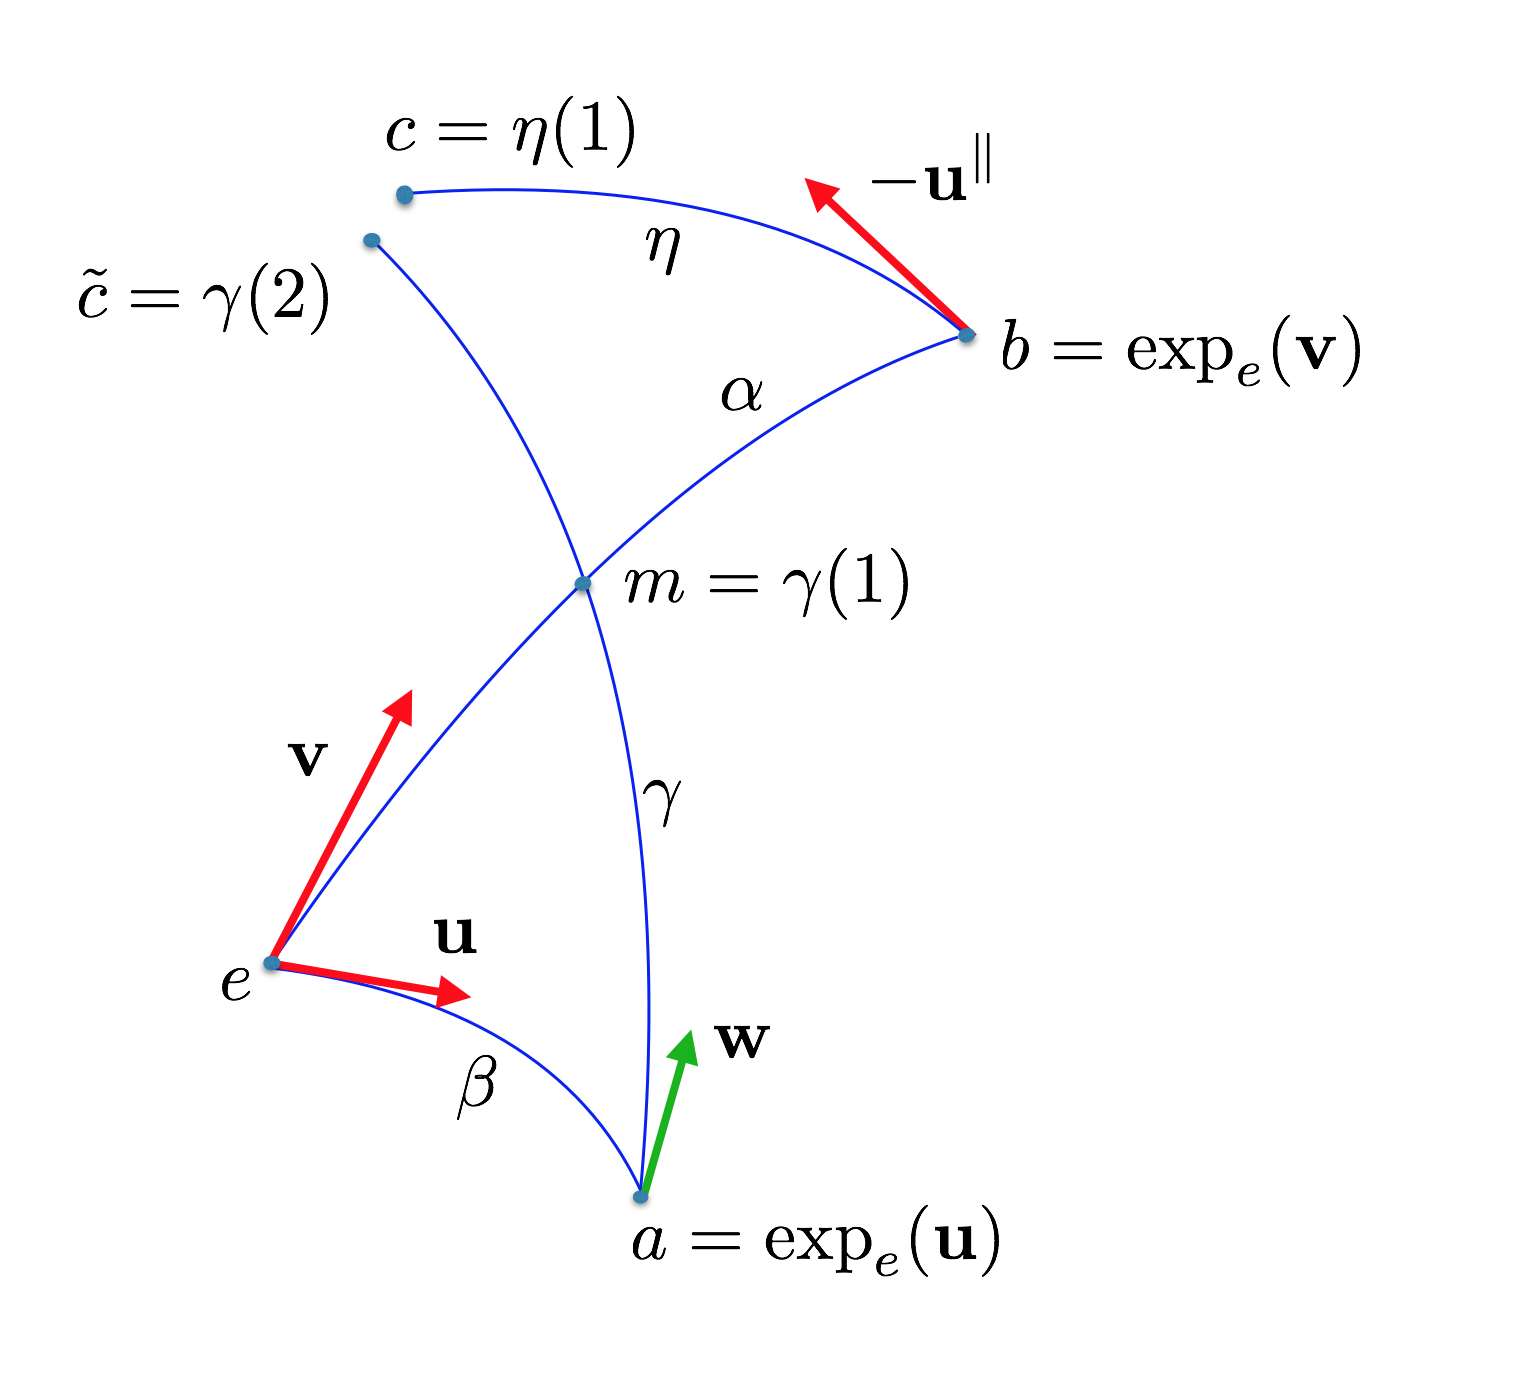
\includegraphics[width=9.5cm]{figures/theorem_pict.png}
	\caption{Pole ladder applied to parallel transport.}
	\label{fig:local}
\end{figure}

\begin{theorem}\label{th:local_approximation_theorem}
	Let $\mathbb{G}$ be a finite dimensional connected Lie group defined with a Cartan connection $\nabla$. 
	If, for each couple of linearly independent vectors $\mathbf{u}, \mathbf{v} \in T_{e}\mathbb{G}$, we consider the following elements:
	\begin{align*}
	a= \exp_{e}(\mathbf{u}) 
	\quad & \quad  
	b= \exp_{e}(\mathbf{v}) \\
	\mathbf{u}^{\parallel} = & \Pi(\alpha)_{e}^{b}(\mathbf{u})\\
	\gamma : [0,1] \rightarrow \mathbb{G} &\quad \gamma(0) = e \quad \dot{\gamma}(0) = \mathbf{v}
	\end{align*}
	Then, for $\mathbf{u}_{e}^{\parallel} := D(L_{b^{-1}})_{e}( -\Pi(\alpha)_{a}^{b}(\mathbf{u}))$, the approximation
	\begin{align*}
	\exp_{e}(\mathbf{u}_{e}^{\parallel}) 
	\simeq
	\exp_{e}\big(\frac{\mathbf{v}}{2}\big)   
	\circ  \exp_{e}(\mathbf{u}) 
	\circ \exp_{e}\big(-\frac{\mathbf{v}}{2}\big)
	\end{align*}
	holds.
\end{theorem}

\begin{proof}
	As a consequence of the construction we have the following considerations:
	\begin{align*}
	\gamma(t) &= \exp(t\mathbf{w}) 
	= 
	a \circ \exp_{e}(D(L_{ba^{-1}})_{e}(t\mathbf{w})) 
	= 
	\exp_{e}(\mathbf{u})  \circ \exp_{e}(D(L_{a^{-1}})_{e}(t\mathbf{w})) 
	\\
	m &= \alpha(\frac{1}{2}) 
	= \exp_{e}\big(\frac{\mathbf{v}}{2}\big) = \gamma(1) = \exp_{a}(\mathbf{w})
	\\
	\exp_{e}&(D(L_{a^{-1}})_{e}(\mathbf{w})) = \exp_{e}(-\mathbf{u}) \circ  \exp_{e}\big(\frac{\mathbf{v}}{2}\big) 
	\end{align*}
	Let $\eta$ be the integral curve of  $-\Pi(\alpha)_{a}^{b}(\mathbf{u})$ starting at $b$. If $c := \eta(1)$ and $\tilde{c} := \gamma(1)$, then on one side we have:
	\begin{align*}
	\tilde{c} = \gamma(1) &= \exp_a(2\mathbf{w}) = a \circ\exp_{e}(D(L_{a^{-1}})_{e}(2\mathbf{w})) \\
	&= \exp_{e}(\mathbf{u})\circ\exp_{e}(D(L_{a^{-1}})_{e}(\mathbf{2w})) \\
	&= \exp_{e}(\mathbf{u})\circ\exp_{e}(2D(L_{a^{-1}})_{e}(\mathbf{w})) \\
	&= \exp_{e}(\mathbf{u})\circ \big(\exp_{e}(D(L_{a^{-1}})_{e}(\mathbf{w})) \big)^2\\
	&=  \exp_{e}(\mathbf{u})\circ \big(  \exp_{e}(-\mathbf{u}) \circ  \exp_{e}(\frac{\mathbf{v}}{2}) \big)^2\\
	&=   \exp_{e}\big(\frac{\mathbf{v}}{2}\big)   
	\circ  \exp_{e}(-\mathbf{u}) 
	\circ \exp_{e}\big(\frac{\mathbf{v}}{2}\big) 
	\end{align*}
	On the other side:
	\begin{align*}
	c = \eta(1) &= \exp_{b}(-\mathbf{u}^{\parallel}) = b \circ\exp_{e}(D(L_{b^{-1}})_{e}(-\mathbf{u}^{\parallel})) \\
	&= \exp_{e}(\mathbf{v}) \circ\exp_{e}(D(L_{b^{-1}})_{e}(-\mathbf{u}^{\parallel})) \\
	&= \exp_{e}(\mathbf{v}) \circ\exp_{e}(-\mathbf{u}_{e}^{\parallel}) 
	\end{align*}
	where $D(L_{b^{-1}})_{e}(\mathbf{u}^{\parallel})$ has been written $\mathbf{u}_{e}^{\parallel}$ for brevity.
	If we consider $c\simeq \tilde{c}$ it follows that:
	\begin{align*}
	\exp_{e}\big(\frac{\mathbf{v}}{2}\big)   
	\circ  \exp_{e}(-\mathbf{u}) 
	\circ \exp_{e}\big(\frac{\mathbf{v}}{2}\big)
	\simeq
	\exp_{e}(\mathbf{v}) \circ\exp_{e}(-\mathbf{u}_{e}^{\parallel}) 
	\end{align*}
	which implies
	\begin{align*}
	\exp_{e}(-\mathbf{u}_{e}^{\parallel}) 
	&\simeq
	\exp_{e}(-\mathbf{v}) 
	\circ \exp_{e}\big(\frac{\mathbf{v}}{2}\big)   
	\circ  \exp_{e}(-\mathbf{u}) 
	\circ \exp_{e}\big(\frac{\mathbf{v}}{2}\big)
	\\
	\exp_{e}(-\mathbf{u}_{e}^{\parallel}) 
	&\simeq
	\exp_{e}\big(-\frac{\mathbf{v}}{2}\big)   
	\circ  \exp_{e}(-\mathbf{u}) 
	\circ \exp_{e}\big(\frac{\mathbf{v}}{2}\big)
	\end{align*}
	As a consequence of property of the signs inversion it follows that
	\begin{align*}
	\exp_{e}(\mathbf{u}_{e}^{\parallel}) 
	\simeq
	\exp_{e}\big(\frac{\mathbf{v}}{2}\big)   
	\circ  \exp_{e}(\mathbf{u}) 
	\circ \exp_{e}\big(-\frac{\mathbf{v}}{2}\big)
	\end{align*}
\end{proof} 

\begin{corollary}
	.... \\
	If, with previous notations, the condition (1) is an approximation
	\begin{align*}
	\exp_{C}(\frac{\mathbf{k}}{2}) = \exp(\mathbf{\xi})\circ \exp_{M}(\frac{\mathbf{k}}{2}) 
	\end{align*}
	for some $ \mathbf{\xi}$ in  $\mathfrak{g}$ such that $\parallel\mathbf{\xi} \parallel < \delta$
	then the approximation has error
	\begin{align*}
	O(\parallel \delta\mathbf{u}^{\parallel} \parallel^{2} )  
	+ O(\parallel \mathbf{u} + \delta\mathbf{u}\parallel^{3})
	+ \text{...something that must be investigated depending on } \delta
	\end{align*}
\end{corollary}


\chapter{Numerical Approximation to Compute the Lie logarithm}\label{ch:lie_log_computation}


% % % % % % % % % % % % % % % % % % % % % % % % % % % % % % % % % % % % % %
% % SUBSECTION
% % % % % % % % % % % % % % % % % % % % % % % % % % % % % % % % % % % % % % 
\section{Exponential and Logarithm Approximation with Truncated Power Series}



% % % % % % % % % % % % % % % % % % % % % % % % % % % % % % % % % % % % % %
% % SUBSECTION
% % % % % % % % % % % % % % % % % % % % % % % % % % % % % % % % % % % % % % 
\section{A reformulation of the Bossa Algorithm using Log-composition}



Having explored some methods to evaluate the BCH formula we can use them to find an approximation of the logarithm function of an element of $\mathbb{G}$. 
Given $p \in \mathbb{G}$ the goal is to find $\mathbf{u}$ such that $\exp(\mathbf{u})$ is the best possible approximation of $p$.  

The first way to find a solution is via the algorithm presented in \cite{Bossa:08}, it reduces the problem of the computation of logarithm to the problem of the computation of the group composition. \\
If $p= \exp(\mathbf{v})$ for any $\mathbf{v} \in \mathfrak{g}$, near the identity we can write:
\begin{align*}
p= \exp(\mathbf{v}) &= (\exp(\mathbf{v})\circ \exp(-\mathbf{v}))\circ \exp(\mathbf{v})\\
&= \exp(\mathbf{v})\circ (\exp(-\mathbf{v})\circ p)\\
&= \exp(\mathbf{v})\circ \exp(\delta \mathbf{v})\\
&\approx \exp(\mathbf{v})\circ \exp(\tilde{\delta} \mathbf{v})
\end{align*}
Where $\tilde{\delta} \mathbf{v}$, as we are going to see, turns out to be $ \exp(-\mathbf{v}) \circ p - e$, for $e$ identity transformation of the Lie group.
The iterative algorithm is then
\begin{equation}\label{eq:bossa_strat}
\begin{cases}
\mathbf{v}_0 = 0 \\
\mathbf{v}_{n} = \text{BCH}^{k}(\mathbf{v}_{n-1},\tilde{\delta} \mathbf{v}_{n-1})
\end{cases}
\end{equation}
for some degree $k$ of approximation.
\begin{align*}
\tilde{\delta} \mathbf{v}_{n-1} =  \exp(-\mathbf{v}_{n-1} )\circ \Phi - e
\end{align*}
%
\begin{proof}  
	Let $\mathbf{v}_{0}$ be an element of $\mathfrak{g}$ in some sense close to $\mathbf{v}$ then:
	\begin{align*}
	p = \exp(\mathbf{v}) &= \exp(\mathbf{v}_{0})\circ (\exp(-\mathbf{v}_{0})\circ p)
	\end{align*}
	We define $\delta \mathbf{v}_{0} \in\mathfrak{g}$ as $\delta \mathbf{v}_{0} = \exp(-\mathbf{v}_{0})\circ p$. Then
	\begin{align*}
	p &= \exp(\mathbf{v}_{0})\circ \exp(\delta \mathbf{v}_{0}) \\
	\exp(V) &= \exp(\mathbf{v}_{0})\circ \exp(\delta \mathbf{v}_{0}) \\
	\mathbf{v} &= \log(\exp(\mathbf{v}_{0})\circ \exp(\delta \mathbf{v}_{0}))\\
	\mathbf{v} &\simeq \text{BCH}^{k}(\mathbf{v}_{0},\delta \mathbf{v}_{0})
	\end{align*}
	We approaching the tangent vector $\mathbf{v}$ using an iterative algorithm based on the $\text{BCH}$ formula and the lemma \ref{le:taylorlemma}.
	\begin{align*}
	\exp(\delta \mathbf{v}_{0}) \approx e + \delta \mathbf{v}_{0} \Longrightarrow \delta \mathbf{v}_{0} \approx  \exp(\delta \mathbf{v}_{0}) - e
	\end{align*}
	Having $\mathbf{v}_{0}$ as our initial value we define
	\begin{align*}
	\tilde{\delta} \mathbf{v}_{0} := \exp(\delta \mathbf{v}_{0}) - e
	\end{align*}
	Using $p = \exp(\mathbf{v}_{0})\circ \exp(\delta \mathbf{v}_{0})$ we can say that $\exp(\delta \mathbf{v}_{0}) =  \exp(-\mathbf{v}_{0})\circ p$ and then
	\begin{align*}
	\tilde{\delta} \mathbf{v}_{0} = \exp(-\mathbf{v}_{0})\circ p - e
	\end{align*}
	just by definition. Since $p$ is known we can start our successive approximation, and if we set $\mathbf{v}_{0} = \mathbf{0}$ we end up with the iterative algorithm (\ref{eq:bossa_strat}).
\end{proof}

\begin{theorem}[Bossa]\label{th:bossa}
	The iterative algorithm (\ref{eq:bossa_strat}) converges to $\mathbf{v}$ with error $\delta_n \in \mathbb{G}$, where
	\begin{align*}
	\delta_{n} := log(\exp(\mathbf{v})\circ \exp(-\mathbf{v}_{n})) \in O(\euclideanMetric{p - e}^{2^{n}})
	\end{align*}
\end{theorem}
%\begin{proof}
%	TODO See notebook or \cite{bossa}.
%\end{proof}

% % % % % % % % % % % % % % % % % % % % % % % % % % % % % % % % % % % % % %
% % SUBSECTION
% % % % % % % % % % % % % % % % % % % % % % % % % % % % % % % % % % % % % % 
\section{Parallel Transport Strategy}

We can use the consideration of the previous section to evaluate the BCH formula in this context, and get an approximation for the evaluation of the Log function.
\begin{align*}
\tilde{\delta} \mathbf{v}_{t-1} = \exp(-\mathbf{v}_{t-1})\circ p - e 
\end{align*}
we get the iterative algorithm
\begin{equation}\label{eq:parallel_strategy}
\begin{cases}
\mathbf{v}_0 = \mathbf{0} \\
\mathbf{v}_{t} = \mathbf{v}_{t-1} - \exp(-\frac{\mathbf{v}_{t-1}}{2}) \circ \exp(\delta \mathbf{v}_{t-1}) \circ \exp(\frac{\mathbf{v}_{t-1}}{2}) + e
\end{cases}
\end{equation}

% % % % % % % % % % % % % % % % % % % % % % % % % % % % % % % % % % % % % %
% % SUBSECTION
% % % % % % % % % % % % % % % % % % % % % % % % % % % % % % % % % % % % % % 
\section{Symmetrization Strategy}

The algorithm for the computation of the group logarithm can be improved considering a symmetric version of the underpinning strategy \ref{eq:bossa_strat}. In this version we use the first order approximation of the BCH formula (see equation (\ref{eq:first_order_approx}) in the following proof), compensating with the fact that the symmetrization should decrease the error involved.
It gives birth to the following algorithm:
\begin{equation}\label{eq:sym_strategy}
\begin{cases}
\mathbf{v}_0 = \mathbf{0} \\
\mathbf{v}_{t+1} = \mathbf{v}_{t} + \frac{1}{2}(\tilde{\delta} \mathbf{v}^{L}_{t} +\tilde{\delta} \mathbf{v}^{R}_{t})
\end{cases}
\end{equation}
Where $\tilde{\delta} \mathbf{v}^{R}_{t} = \exp(\mathbf{v})\circ \exp(- \mathbf{v}_{t}) - e$ and $\tilde{\delta} \mathbf{v}^{L}_{t} = \exp(-\mathbf{v}_{t})\circ \exp(\mathbf{v}) - e$.\\
\begin{proof}
	To show why it works we remind that the starting point was
	\begin{align*}
	p= \exp(\mathbf{v}) &=  \exp(\mathbf{v}_{0})\circ \exp(\delta \mathbf{v}_{0})
	\end{align*}
	where $\exp(\delta \mathbf{v}_{0}) = \exp(-\mathbf{v}_{0})\circ p$.\\
	An equivalent starting point would have been $\exp(\mathbf{v}) = \exp(\delta \mathbf{v})\circ \exp(\mathbf{v}_{0})$ for $\exp(\delta \mathbf{v}) = p\circ \exp(-\mathbf{v}_{0})$. \\
	This idea leads to the definition of
	\begin{align*}
	\exp(\delta \mathbf{v}^{R}_{t}) &:= p\circ \exp(- \mathbf{v}_{t}) = \exp(\mathbf{v})\circ \exp(- \mathbf{v}_{t})\\
	\exp(\delta \mathbf{v}^{L}_{t}) &:=  \exp(- \mathbf{v}_{t}) \circ p = \exp(- \mathbf{v}_{t}) \circ \exp(\mathbf{v}) 
	\end{align*}
	It follows that 
	\begin{align*}
	\exp(\mathbf{v}) &= \exp(\mathbf{v}_{0})\circ \exp(\delta \mathbf{v}^{R}_{0})\\
	\exp(\mathbf{v}) &=  \exp(\delta \mathbf{v}^{L}_{0}) \circ \exp(\mathbf{v}_{0})
	\end{align*}
	Using $\exp(\delta \mathbf{v}^{R}_{t}) \approx e + \delta \mathbf{v}^{R}_{t}$ and $\exp(\delta \mathbf{v}^{L}_{t}) \approx e + \delta \mathbf{v}^{L}_{t}$ we can use the following approximation to define the symmetric algorithm:
	\begin{align*}
	\exp(\delta \mathbf{v}^{R}_{t}) &= \exp(\mathbf{v})\circ \exp(-\mathbf{v}_{t})\\
	e + \tilde{\delta} \mathbf{v}^{R}_{t} &= \exp(\mathbf{v})\circ \exp(- \mathbf{v}_{t})\\
	\tilde{\delta} \mathbf{v}^{R}_{t} &= \exp(\mathbf{v})\circ \exp(- \mathbf{v}_{t}) - e
	\end{align*}
	\begin{align*}
	\exp(\delta \mathbf{v}^{L}_{t}) &= \exp(- \mathbf{v}_{t}) \circ \exp(\mathbf{v})\\
	e + \tilde{\delta} \mathbf{v}^{L}_{t} &= \exp(-\mathbf{v}_{t})\circ \exp( \mathbf{v})\\
	\tilde{\delta} \mathbf{v}^{L}_{t} &= \exp(-\mathbf{v}_{t})\circ \exp(\mathbf{v}) - e
	\end{align*}
	Which gives birth to iterative algorithm, for a given initial value $V_0$:  
	\begin{equation}
	\begin{cases}
	\mathbf{v}_0  \\
	\mathbf{v}_{t+1} =\text{BCH}(\mathbf{v}_{t},\tilde{\delta} \mathbf{v}^{R}_{t})
	\end{cases}
	\begin{cases}
	\mathbf{v}_0  \\
	\mathbf{v}_{t+1} = \text{BCH}(\tilde{\delta} \mathbf{v}^{L}_{t}, \mathbf{v}_{t})
	\end{cases}
	\end{equation}
	If follows that
	\begin{align*}
	\mathbf{v}_{t+1} = \frac{1}{2}(\text{BCH}(\tilde{\delta} \mathbf{v}^{L}_{t}, \mathbf{v}_{t}) + \text{BCH}(\mathbf{v}_{t},\tilde{\delta} \mathbf{v}^{R}_{t}))
	\end{align*}
	Taking the first order approximation of the BCH formula:
	\begin{align}\label{eq:first_order_approx}
	BCH(\tilde{\delta} \mathbf{v}^{L}_{t}, \mathbf{v}_{t}) &\approx \tilde{\delta} \mathbf{v}^{L}_{t} + \mathbf{v}_{t}\\
	BCH(\mathbf{v}_{t},\tilde{\delta} \mathbf{v}^{R}_{t}) &\approx \mathbf{v}_{t} + \tilde{\delta} \mathbf{v}^{R}_{t}
	\end{align}
	we get
	\begin{align*}
	\mathbf{v}_{t+1} = \mathbf{v}_{t} + \frac{1}{2}(\tilde{\delta} \mathbf{v}^{L}_{t} + \tilde{\delta} \mathbf{v}^{R}_{t})
	\end{align*}
\end{proof}
We observe that the symmetric approach do not requires to use the BCH formula at each passage, having considered the approximation at the first order of the BCH.\\
We conclude with a formula that relates $\tilde{\delta} \mathbf{v}^{L}_{t}$ with $\tilde{\delta} \mathbf{v}^{R}_{t}$:
\begin{theorem}
	Be $\tilde{\delta} \mathbf{v}^{R}_{t} = \exp(\mathbf{v})\circ \exp(- \mathbf{v}_{t}) - e$ and $\tilde{\delta} \mathbf{v}^{L}_{t} = \exp(-\mathbf{v}_{t})\circ \exp(\mathbf{v}) - e$ as before, then
	\begin{align*}
	\delta \mathbf{v}^{L}_{t} \approx \exp(-\mathbf{v}_{t}) \circ \delta \mathbf{v}^{R}_{t} \circ \exp(\mathbf{v}_{t})
	\end{align*}
\end{theorem}
\begin{proof}
	Since $\exp(\mathbf{v}_{t})\circ \exp(\delta \mathbf{v}^{R}_{t}) \approx exp(\delta \mathbf{v}^{L}_{t}) \circ \exp(\mathbf{v}_{t})$ it follows
	\begin{align*}
	\exp(\delta \mathbf{v}^{R}_{t}) = \exp(-\mathbf{v}_{t})\circ \delta \mathbf{v}^{L}_{t} \circ \exp(\mathbf{v}_{t})
	\end{align*}
	Using $\exp(\delta \mathbf{v}^{R}_{t}) = e + \delta \mathbf{v}^{R}_{t}$ and $\exp(\delta \mathbf{v}^{L}_{t}) = e + \delta \mathbf{v}^{L}_{t}$ we get
	\begin{align*}
	e + \delta \mathbf{v}^{R}_{t} &= \exp(-\mathbf{v}_{t})\circ (e + \delta \mathbf{v}^{L}_{t}) \circ \exp(\mathbf{v}_{t})\\
	\delta \mathbf{v}^{R}_{t} &= \exp(-\mathbf{v}_{t})\circ \delta \mathbf{v}^{L}_{t} \circ \exp(\mathbf{v}_{t})
	\end{align*}
\end{proof}

% % % % % % % % % % % % % % % % % % % % % % % % % % % % % % % % % % % % % %
% % SUBSECTION
% % % % % % % % % % % % % % % % % % % % % % % % % % % % % % % % % % % % % %
\section{Symmetric-Parallel Transport Strategy}
If we are not satisfied to having take only the firs order approximation of the BCH in the equation (\ref{eq:first_order_approx}) we use at this stage the parallel transport in the method presented in this section.
Going back to the algorithm \ref{eq:sym_strategy} we can apply to
\begin{align*}
\mathbf{v}_{t+1} = \frac{1}{2}(\text{BCH}(\tilde{\delta} \mathbf{v}^{L}_{t}, \mathbf{v}_{t}) + \text{BCH}(\mathbf{v}_{t},\tilde{\delta} \mathbf{v}^{R}_{t}))
\end{align*}
the parallel transport to get
\begin{align*}
\mathbf{v}_{t+1} &= \frac{1}{2}((\tilde{\delta} \mathbf{v}^{L}_{t})^{\parallel} + \mathbf{v}_{t} + \mathbf{v}_{t} + (\tilde{\delta} \mathbf{v}^{R}_{t})^{\parallel}) \\
&= 2\mathbf{v}_{t} + \frac{1}{2}((\tilde{\delta} \mathbf{v}^{L}_{t})^{\parallel} + (\tilde{\delta} \mathbf{v}^{R}_{t})^{\parallel})
\end{align*}
Applying the definition of parallel transport we get
\begin{align*}
(\tilde{\delta} \mathbf{v}^{L}_{t})^{\parallel} + (\tilde{\delta} \mathbf{v}^{R}_{t})^{\parallel} 
= 
\exp(-\frac{\mathbf{v}_{t}}{2}) \circ (\tilde{\delta} \mathbf{v}^{L}_{t} +\tilde{\delta} \mathbf{v}^{R}_{t} )\circ \exp(\frac{\mathbf{v}_{t}}{2})
\end{align*}
where 
\begin{align*}
\tilde{\delta} \mathbf{v}^{L}_{t} &=  \exp(\mathbf{v})\circ \exp(-\mathbf{v}_{t}) - e \\
\tilde{\delta} \mathbf{v}^{R}_{t} &=  \exp(-\mathbf{v}_{t})\circ \exp(\mathbf{v}) - e
\end{align*}
Then a new improvement of the algorithm \ref{eq:bossa_strategy}  is
\begin{equation}\label{eq:sym_parallel_strategy}
\begin{cases}
\mathbf{v}_0 = 0 \\
\mathbf{v}_{t} 
=  
2\mathbf{v}_{t-1} + \frac{1}{2}(\exp(-\frac{\mathbf{v}_{t-1}}{2}) 
\circ 
(\tilde{\delta} \mathbf{v}^{L}_{t-1} +\tilde{\delta} \mathbf{v}^{R}_{t-1} )\circ \exp(\frac{\mathbf{v}_{t-1}}{2}))
\end{cases}
\end{equation}
(This must be investigated!)
\chapter{Experimental Results}\label{ch:results}

\begin{flushright}
	\emph{\lq\lq A victory is twice itself when the achiever brings home full numbers.\rq\rq \\
		       \emph{Much ado about nothing}, Leonato, scene 1.}
\end{flushright}


% % % % % % % % % % % % % % % % % % % % % % % % % % % % % % % % % % % % % %
% % SUBSECTION
% % % % % % % % % % % % % % % % % % % % % % % % % % % % % % % % % % % % % % 



\section{Log-composition for SE(2)}


\subsection{Methods}

\subsection{Results}

%\subsection{Log-Compositions Performance for Toy examples and Patient Images}


\section{Log-composition for SVF}

\subsection{Methods}

\subsection{Results}

\section{Log-computation Algorithm}

\subsection{Methods}

\subsection{Results}

\section{Further Research and Conclusion}\label{ch:conclusions}


Considering only the results, this one-year research can be considered much ado about nothing, but...


% % % % % % % % % % % % % % % % % % % % % % % % % % % % % % % % % % % % % %
% % % % % % % % % % % % % % % % % % % % % % % % % % % % % % % % % % % % % %
% % % % % % % % % % % % % % % % % % % % % % % % % % % % % % % % % % % % % % 
\chapter{Conclusions}\label{ch:conclusions}

In this research we have formally defined the mathematical concept of Lie log-composition and we have presented the limitations of the numerical methods for its computation obtained with truncations of the BCH formula. These limitations are the starting point of the research for BCH-free numerical methods. 
One of these, based on the geometrical concept of parallel transport is presented here for the first time, and formally proved for element of the general Lie algebra.

This method is compared with the truncated BCH, both for elements belonging to the the Lie algebra of rigid body transformations (where also another BCH-free numerical method based on the Taylor expansion is available) and for stationary velocity fields (SVF).

The possible applications of efficient numerical methods for the computation of the Lie log-composition in medical imaging are listed in section \ref{se:applications_log_com_in_med}. One of these, the computation of the Lie logarithm based on the algorithm presented in \cite{bossa2008new}, is investigated in chapter \ref{ch:log_algorithm}.

Results show that the Lie log-composition computed with the parallel transport method improves the $\text{BCH}^0$, and gets, in general close to the $\text{BCH}^1$. At an higher computational cost it enable to avoid the computation of the Jacobian involved in the $\text{BCH}^1$, obtaining results more precise than the $\text{BCH}^0$ when the vectors involved are considered have norm in a limited range.

Results show also that for medical applications is not recommendable to utilize numerical approximations based on $\text{BCH}^k$ for $k\geq 2$. The method that provides best results both on synthetic and real data on a wider range of SVF, is the $\text{BCH}^1$, that involves one nested Lie bracket. The parallel transport is the first choice (and the unique at the moment) when it is preferable to avoid the computation of the Lie bracket. 


% % % % % % % % % % % % % % % % % % % % % % % % % % % % % % % % % % % % % %
% % % % % % % % % % % % % % % % % % % % % % % % % % % % % % % % % % % % % % 
\section{Further Researches}\label{se:further_research}

Since this thesis has both numerical and theoretical aspects, improvements could be reached with a better understanding of both sides.

\subsection{Numerical Computations} 

Numerical computations on real data for small SVF, provide better results for parallel transport than for any other available numerical method (see figure \ref{fig:svf_log_composition_real_data_CTL_expo}) when the norm of the elements involved are smaller than $0.0227$. The reason why this does not happen for synthetic data may be due to the fact that the Jacobian determinant of SVF are not always positive, when in particular for SVF with small norm. This may lead to consider better way to generating random SVF than the one proposed in this research. 

To compute the Lie exponential and the Lie logarithm we always used the scaling and squaring and the inverse scaling and squaring algorithms, as originally proposed by Arsigny in $2006$ \cite{arsigny2006log}. There are other options available that, when applied to the log-composition, could improve the computational time. These are based for example on the Euler method, the midpoint method, the modified Euler method and Runge-Kutta of order $4$. Investigations in this direction are currently in progress.

The proof of the convergence for the BCH in Dynkin's paper is based on the power series expansion of the exponential and of the logarithm (equation (\ref{eq:exp_as_inf_sum}) and (\ref{eq:log_as_inf_sum}))
but these expansions, unless using the function $\mathcal{V}$ proposed in section \ref{subse:bigger_algebra} are not well defined, and have never been proved for the Lie algebra of diffeomorphisms.
Numerical tests, on which we are currently working, seem to show that the Lie exponential computed with the expansion in power series converges for SVF.

\subsection{Theoretical Formulas}

Certainly not all of the possibilities provided by the application of the concept of parallel transport for the computation of the Lie log-composition have been exploited. The formula (\ref{eq:parallel_transport}), presented at the end of chapter \ref{ch:tools}, can still be improved, for example finding strategies to reduce the number of underpinning assumptions and introducing some numerical techniques to compute the Affine exponential. When this tool will be available, formula (\ref{eq:parallel_transport}) could be reformulated as
\begin{align*}
\mathbf{u}\oplus \mathbf{v}
&\simeq
\exp_{\exp(\mathbf{u} )}(\mathbf{v} ) - e
\end{align*} 
or, in a symmetric version,  as
\begin{align*}
\mathbf{u}\oplus \mathbf{v}
&\simeq
\frac{1}{2}
\big(
\exp_{\exp(\mathbf{u} )}(\mathbf{v} ) 
+
\exp_{\exp(\mathbf{v} )}(\mathbf{u} )
\big)
-  e
\end{align*} 

Another BCH-free formula, not based on the parallel transport, could be obtained finding a way to extend the Taylor expansion proposed for $SE(2)$ in section \ref{se:rigid_body_transformations} to SVF.

A third one, on which  preliminary tests showed promising results, is obtained using the accelerating convergence series \cite{cohen2000convergence} on the series expansion of the Lie exponential and the Lie logarithm. This is based on the assumption that Lie logarithm and Lie exponential are analytic also for SVF.




%%%%%%%%%%%%% Appendice  %%%%%%%%%%%%%%%%%%%%%%%%%%%
%%%%%%%%%%%%%%%%%%%%%%%%%%%%%%%%%%%%%%%%%%%%%%%%

\pagestyle{plain}

\addcontentsline{toc}{chapter}{Appendices}

% The \appendix command resets the chapter counter, and changes the chapter numbering scheme to capital letters.
%\chapter{Appendices}
\appendix
%\chapter{An Appendix About Stuff}
%\label{appendixlabel1}
%(stuff)
%
%\chapter{Another Appendix About Things}
%\label{appendixlabel2}
%(things)

\section*{Appendix: NiftyReg and NiftyBit}
\label{appendixlabel3}
xxx  This will be a short a description of the tools you used to make experiments for this thesis. 

%%%%%%%%%%%%% BIBLIOGRAFIA  %%%%%%%%%%%%%%%%%%%%%%%%%%%
%%%%%%%%%%%%%%%%%%%%%%%%%%%%%%%%%%%%%%%%%%%%%%%%
\newpage
\bibliography{frontback/mres_bib.bib}
\bibliographystyle{alpha}
\end{document}